% REMEMBER: You must not plagiarise anything in your report. Be extremely careful.

\documentclass{l4proj}

    
%
% put any additional packages here
%

\begin{document}

%==============================================================================
%% METADATA
\title{Emulating Glasgow's First Computer}
\author{Gerard Ward}
\date{March 25, 2019}

\maketitle

%==============================================================================
%% ABSTRACT
\begin{abstract}
    The English Electric DEUCE was one of the first commercially available computers in the world,
	but in modern times, there are limited resources available to learn more about it. The aim of
	this project was to create an emulator of the DEUCE, to provide people with a way of learning
	how one of the world's earliest computers functions. Written as a web application, this emulator
	allows users to operate the DEUCE as if they were using an original, but through a modern software
	solution. In the end, the project captured most of the functionality of the original DEUCE.
\end{abstract}

%==============================================================================

% EDUCATION REUSE CONSENT FORM
% If you consent to your project being shown to future students for educational purposes
% then insert your name and the date below to  sign the education use form that appears in the front of the document. 
% You must explicitly give consent if you wish to do so.
% If you sign, your project may be included in the Hall of Fame if it scores particularly highly.
%
% Please note that you are under no obligation to sign 
% this declaration, but doing so would help future students.
%
\def\consentname {Gerard Dominic Ward} % your full name
\def\consentdate {20 March 2018} % the date you agree
%
\educationalconsent


%==============================================================================
\tableofcontents

%==============================================================================
%% Notes on formatting
%==============================================================================
% The first page, abstract and table of contents are numbered using Roman numerals and are not
% included in the page count. 
%
% From now on pages are numbered
% using Arabic numerals. Therefore, immediately after the first call to \chapter we need the call
% \pagenumbering{arabic} and this should be called once only in the document. 
%
% The first Chapter should then be on page 1. You are allowed 40 pages for a 40 credit project and 20 pages for a 
% 20 credit report. This includes everything numbered in Arabic numerals (excluding front matter) up
% to but excluding the appendices and bibliography.
%
% You must not alter text size (it is currently 10pt) or alter margins or spacing.
%
%
%==================================================================================================================================
%
% IMPORTANT
% The chapter headings here are **suggestions**. You don't have to follow this model if
% it doesn't fit your project. Every project should have an introduction and conclusion,
% however. 
%
%==================================================================================================================================
\chapter{Introduction}

% reset page numbering. Don't remove this!
\pagenumbering{arabic} 
This chapter states the motivations and aims behind this project, as well as summarising the
contents of the rest of this dissertation. The DEUCE emulator built for this project allows
users to operate a web application version of the English Electric DEUCE. The significance of creating
this emulator will be explained in this chapter.

\section{Motivation}

In 1951, the English Electric company decided to begin building models of the Digital Electronic Universal Computing Engine, also known as the DEUCE \citep{Vowels05}. This computer was based on Alan Turing's Pilot ACE computer but improved on the ACE in several ways, namely by improving upon the speed and reliability of the ACE, adding further storage and adding a large program and subroutine library. Due to these improvements, the DEUCE was considered a success: in total, approximately 33 DEUCEs were created, with the first being made commercially available in 1955. \citep{Vowels05}. DEUCEs were mainly installed at governmental departments, aircraft design facilities and universities. Therefore, as an early, commercially successful stored program computer, the DEUCE has a hugely important part in the history of Computing Science.

Among the universities that installed a DEUCE was the University of Glasgow \citep{Glasgow60}. In 1957, the university established Scotland's first computing lab and chose Dr. Dennis Gilles as its initial Director of Computing, as pictured in Figure \ref{fig:gilles}. As director, Gilles was responsible for advising the university to order its first computer and so in 1958, the DEUCE became the first electric computer at a Scottish university. In addition to holding an important place in the history of Computing Science, the DEUCE is also significant in recent Scottish academic history.

\begin{figure}[b]
	\centering
	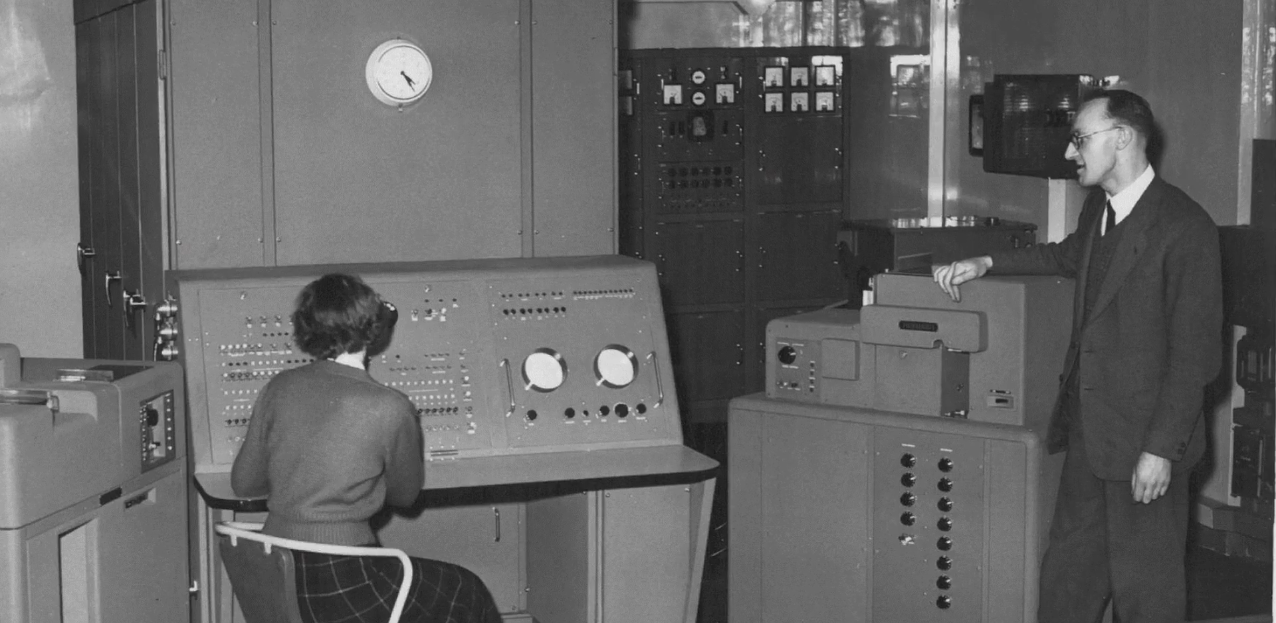
\includegraphics[width=0.7\linewidth]{images/gilles}
	\caption{DEUCE operator Anne Low with Dr. Dennis Gilles, initial Director of Computing at the University of Glasgow, c. 1957. \citep{DelayLine19}}
	\label{fig:gilles}
\end{figure}

However, in spite of the DEUCE's importance as an early electric computer, there remain limited resources available on the DEUCE today. With all of the machines having stopped being in use since approximately the late 1960s, there are no DEUCEs left to operate in the world today. At the University of Glasgow, the only remaining piece of the DEUCE that was installed is one of the mercury delay lines, as shown in Figure \ref{fig:amp}. For this reason, it would be beneficial if there were a modern way of allowing people to operate a DEUCE. This would let them learn more about an important part of Computing Science history, as well as allowing them to learn how to operate an example of an early computer.

\begin{figure}[h!]
	\centering
	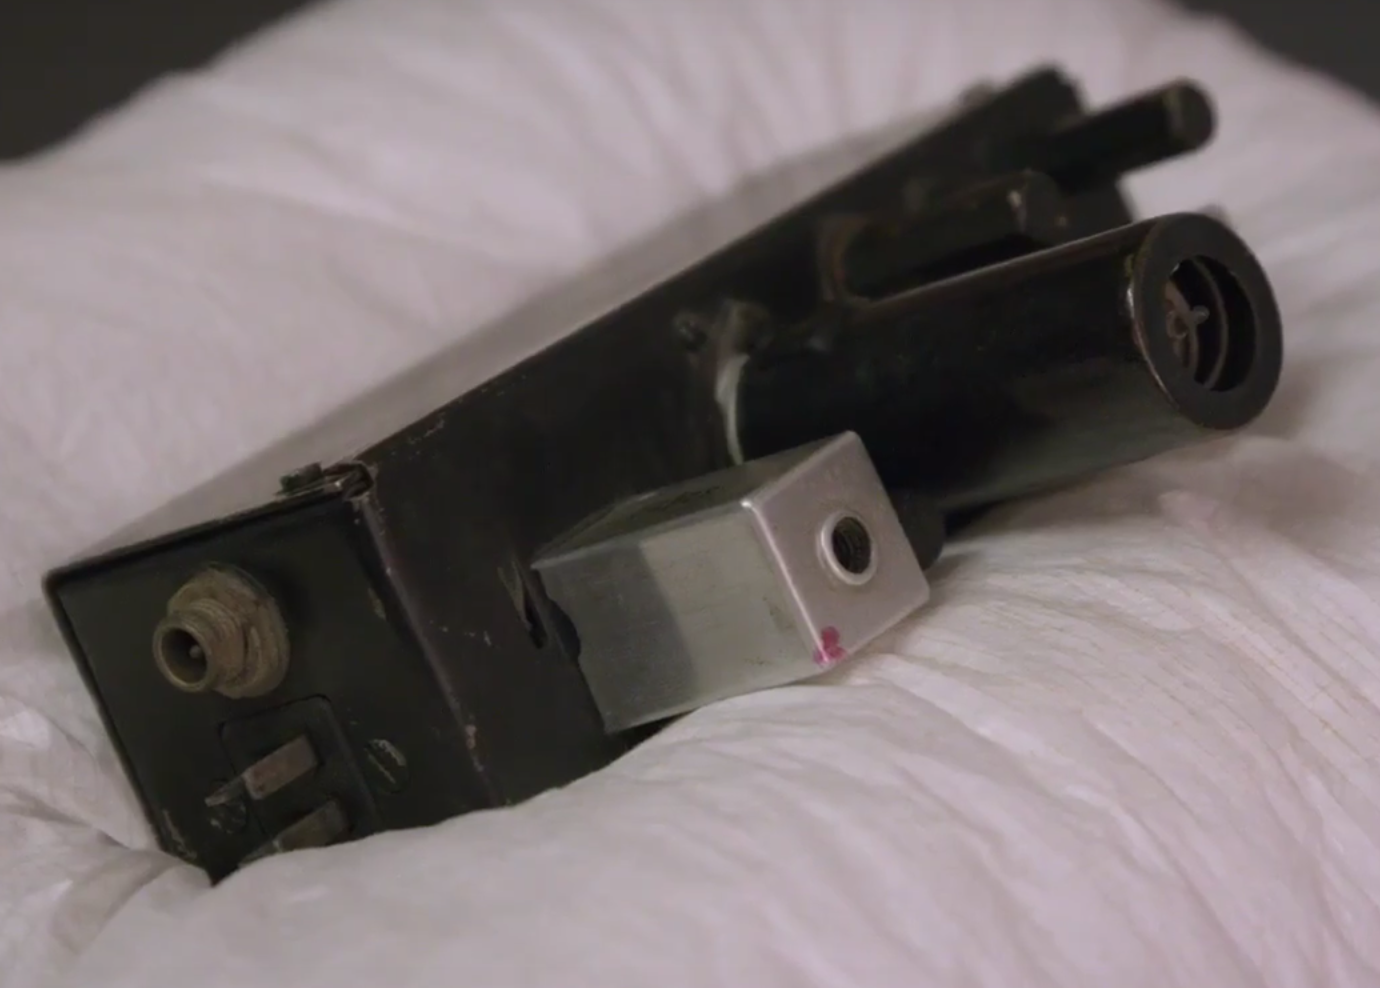
\includegraphics[width=0.7\linewidth]{images/delay-line-amplifier}
	\caption{Mercury delay line amplifier from original Glasgow DEUCE. This piece of equipment sent electrical pulses to encode data inside the mercury delay lines of the DEUCE. \citep{DelayLine19}}
	\label{fig:amp}
\end{figure}


In modern times, it would be impractical to recreate the DEUCE physically. With the DEUCE drawing around 9kW of power and having a clock speed of 1MHz \citep{Glasgow60}, it is a highly inefficient system. Furthermore, its use of mercury delay lines would be dangerous given the potential health problems associated with exposure to mercury \citep{Gao17}. Therefore, an alternative way of recreating the DEUCE in modern times would be through emulation. According to \citet{Nair05}, emulation is "the process of implementing the interface and functionality of one system or subsystem on a system or subsystem having a different interface and functionality." The creation of a DEUCE emulator would be a modern, efficient and convenient way for the DEUCE to be remade and would solve the problem of the DEUCE being widely unavailable to people.

\section{Aims}

For this project, the key aim is to create a functioning emulator of the DEUCE. The emulator should replicate the behaviour of the original DEUCE, using the same input, processing and output methods. When completed, the emulator should allow the user to run programs on it, as if it were the original DEUCE computer. It should also replicate the user interface of the DEUCE. After the emulator has been created, it should be evaluated against the original DEUCE to discover if it can run programs written for the original computer. It is hoped that the emulator can be used as an educational tool to help people learn more about how early computers, such as the DEUCE, functioned.

\section{Summary}

The purpose of this chapter was to introduce they key motivations behind the project and what the aims of the project should be. The rest of this dissertation will be structured as follows:

\begin{itemize}
	\item Chapter 2 will examine the background research carried out on how the DEUCE functioned. It will also examine similar early computer emulators and look into what made these emulators examples of good or bad emulators.
	\item Chapter 3 will examine the requirements gathering process for the emulator and the choices behind the target platform chosen for the project.
	\item Chapter 4 will examine the initial design choices made for the emulator and the decisions which informed the design of both the graphical and system design of the computer.
	\item Chapter 5 will discuss the implementation process of the project and how the frontend and backend of the project was implemented.
	\item Chapter 6 will examine how the emulator was evaluated against the original DEUCE, to discover how successful it was in emulating its behaviour.
	\item Chapter 7 will reflect on possible future steps for the project and what could have been improved about the emulator. 
\end{itemize}

%==================================================================================================================================
\chapter{Background}
This chapter discusses background research carried out on the DEUCE and on the creation of emulators. Research into both of these topics was necessary to fully understand how to create a DEUCE emulator. Using the research undertaken in this chapter, it was easier to make informed decisions later in the software development process for the DEUCE emulator.

\section{Learning how the DEUCE functions}
\begin{figure}[h!]
	\centering
	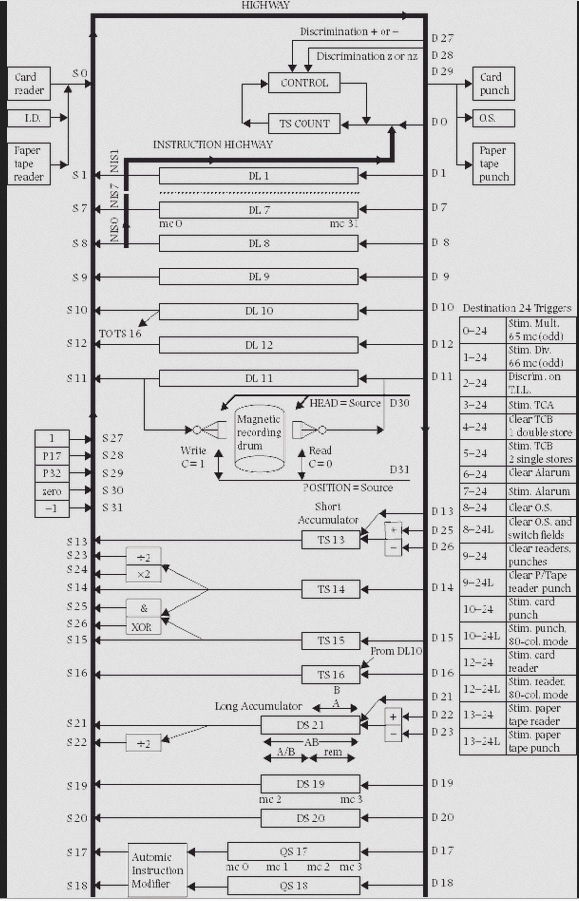
\includegraphics[width=0.5\linewidth]{images/deuce-arch.jpg} 
	\caption{Architecture diagram of the DEUCE \citep{Vowels05}. This image shows the memory structure of the delay lines, registers and special memory locations used to carry out special functions in the DEUCE.}
	\label{fig:arch}
\end{figure}

Firstly, it was important to learn how the DEUCE functioned as a computer. The architecture of the DEUCE is shown in Figure \ref{fig:arch}. As an early computer, it is extremely different to modern computers in several ways. For example, for input, the instructions read in by the DEUCE were essentially a series of move instructions from a memory source to a memory destination. Each instruction was a 32-bit binary word \citep{Weth10}. Instructions could be read in either via a card reader, which read in lines of instructions on special punch cards, or through the Input Dynamiciser, a special row of switches which allowed for single word input. Several special source and memory locations were used for special functions, such as arithmetic functions, discrimination functions etc., and through using these special memory locations, the computer could be coded to run programs.

The DEUCE stored instructions in delay lines and registers. It consisted of:
\begin{itemize}
	\item 32 mercury delay lines, each storing 32 words.
	\item 4 Temporary Store registers, each storing 1 word.
	\item 3 Double Store registers, each storing 2 words.
	\item 2 Quadruple Store registers, each storing 4 words.
\end{itemize}	
For output, the DEUCE could display information through the Output Staticiser, which was a row of lights that could display a single 32-bit word, or through a screen which could display a matrix of bits.

The complex mechanics of the DEUCE meant that the architecture of the computer had to be studied carefully in order to fully understand how to emulate its behaviour.

\section{Comparison of early computer emulators}
To gain a better understanding of how early computers worked, several emulators of other early computers were researched. This gave good insight into how similar early computers functioned and allowed for the exploration of the design choices behind these emulators.

\subsection{Pilot ACE Emulator} 
\begin{figure}[h]
	\centering
	\begin{subfigure}[t]{0.45\textwidth}
		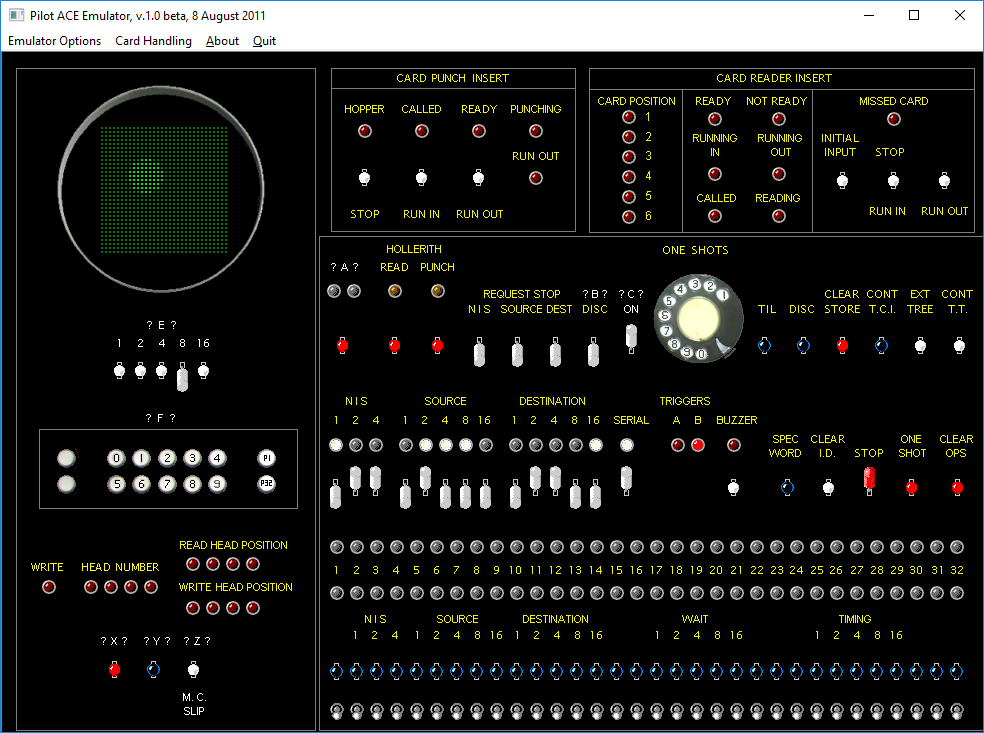
\includegraphics[width=\textwidth]{images/ace-emulator}
		\caption{Pilot ACE Emulator from pilotaceonline.com \citep{Ace12}, accessed using Wayback Machine \citep{Wayback19}. This image shows the emulator console featuring switches and lights used for input and output respectively. It also shows the toolbar used for entering CRD "punch card" files and a monitor for displaying output.}
		\label{fig:ace-emu}
	\end{subfigure}
	\quad
	~ %add desired spacing between images, e. g. ~, \quad, \qquad, \hfill etc. 
	%(or a blank line to force the subfigure onto a new line)
	\begin{subfigure}[t]{0.45\textwidth}
		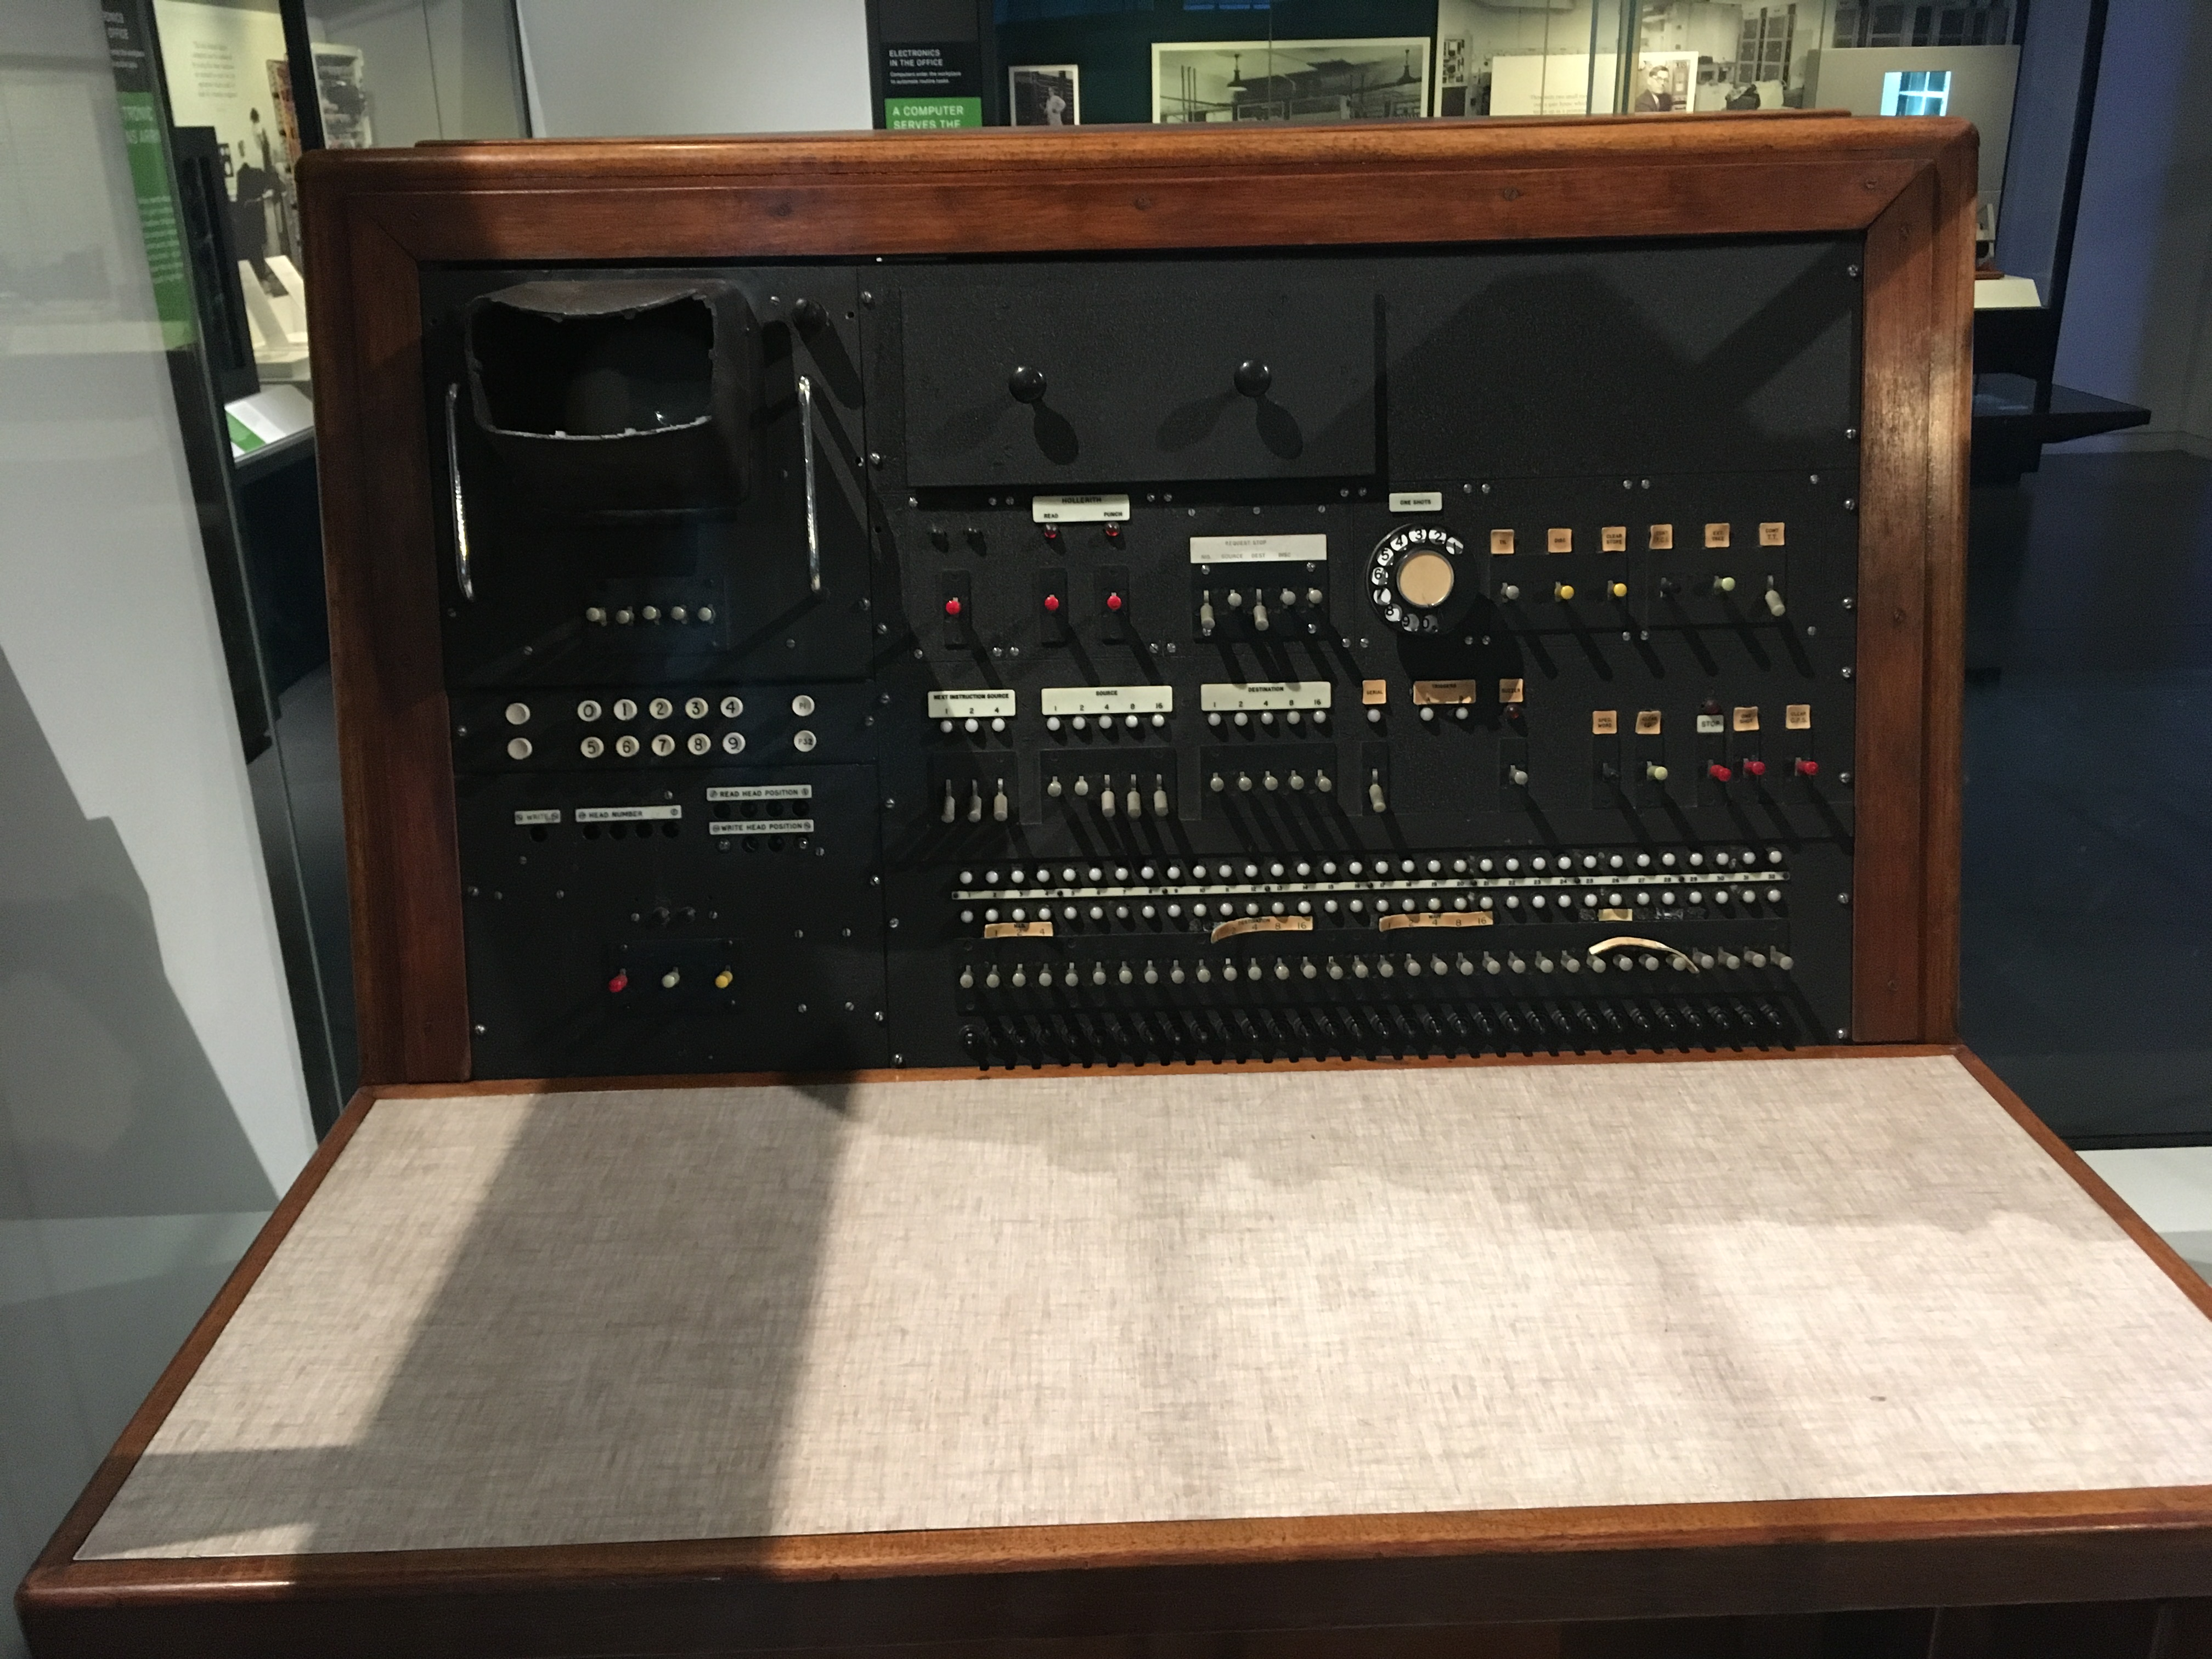
\includegraphics[width=\textwidth]{images/real-ace}
		\caption{Image of console from real Pilot ACE, taken at Science Museum, London. Emulator shown in Figure \ref{fig:ace-emu} strongly resembles real front panel of the machine.}
		\label{fig:real-ace}
	\end{subfigure}
	~ %add desired spacing between images, e. g. ~, \quad, \qquad, \hfill etc. 
	%(or a blank line to force the subfigure onto a new line)    
	\caption{Images of Pilot ACE emulator by David Green and the original Pilot ACE machine at the Science Museum, London.}
	\label{fig:ace-comps}
\end{figure}
As described by \citet{VowelsAce05}, the Pilot ACE was one of the earliest stored-program computers and was based on a design by Alan Turing, running its first program in 1950. The DEUCE was a commercial version of this machine, so there are several similarities between the two computers. For example, both machines can read input from a Hollerith card reader or from the Input Dynamiciser keys on the front panel of the machine. The main memory of the Pilot ACE consisted of 11 32-bit delay lines, 5 32-bit temporary stores and 2 64-bit double stores.

This emulator, as seen in Figure \ref{fig:ace-emu}, is a very faithful recreation of the original Pilot ACE, as seen in Figure \ref{fig:real-ace}. The panel is a replica of the original panel of the Pilot ACE. To recreate some of the physical actions of operating the Pilot ACE, such as inserting a card into the card reader, the author instead provides a toolbar that allows some of these features to be carried out.

Therefore, the Pilot ACE emulator is a very useful model on which to base a DEUCE emulator. Given the similarities in how the Pilot ACE and DEUCE computers functioned, this emulator provided some very good ideas about how to implement a DEUCE emulator. As the DEUCE was a commercial version of this machine, many of the features present in this emulator can be reused in a DEUCE emulator, such as the input dynamiciser and single shot key. While the GUI is an accurate representation of the original Pilot ACE interface, several of the features of the original Pilot ACE appear unknown to the author. For example, the purposes of the keys surrounded by question marks, such as "? E ?", are unknown to the creator. Overall, it would be worthwhile to base several features of a DEUCE emulator on this emulator.


\subsection{The EDSAC Simulator}
\begin{figure}[h!]
	\centering
	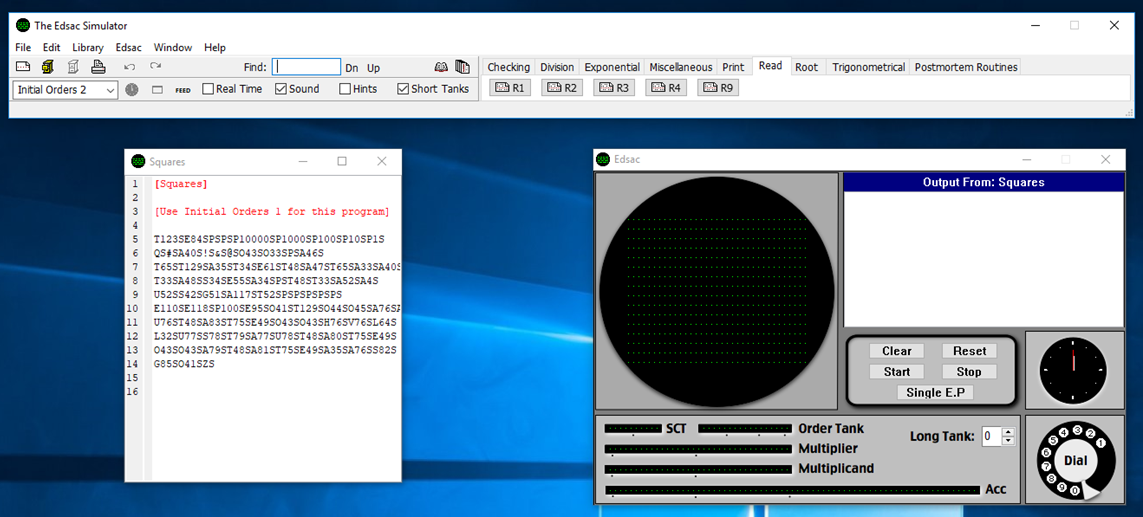
\includegraphics[width=\linewidth]{images/edsac-emu}
	\caption{EDSAC Simulator from the University of Warwick \citep{Warwick16}. Image shows the toolbar, program text and simulator display.}
	\label{fig:edsac}
\end{figure}

Like the Pilot ACE and the DEUCE, the EDSAC was another early stored program computer. Its functionality is described by \citet{Edsac11}. Running its first program in 1949, it used 32 mercury delay lines for main memory, each storing 32 words of 18 bits. For input, it used a paper-tape reader operating at 50 characters per second and output was achieved through a Creed teleprinter. Control can be achieved through five buttons: clear, reset, start, stop and single E.P. Single E.P functions similarly to the single shot key in the DEUCE, by allowing a program to be executed one instruction at a time. 

As shown in Figure \ref{fig:edsac}, the EDSAC emulator has three main components: the toolbar, the program text and the simulator display. The toolbar allows control over the features of the EDSAC. For example, it allows files to be read in and allows the user to switch between Initial Orders 1 and Initial Orders 2. The program text provides the series of instructions to be executed for a program that is being read in. The simulator display shows the output from the programs being executed and allows control over programs through the five main control buttons.

Overall, while there are bigger differences between the DEUCE and the EDSAC than the DEUCE and the Pilot ACE, this is still a useful emulator on which to model some features of the DEUCE. Both computers share common features such as using a reader to take input from files and using delay lines for main memory. One useful feature of this emulator compared to the Pilot ACE emulator is its output display. Rather than outputting to a new file, it is useful to have a console that displays output instead. This would be a good feature to have in a DEUCE emulator, particularly one running as a web app. Therefore, while several features would need to change, there are some features of this emulator that would be useful to base a DEUCE emulator on.

\subsection{Manchester Baby Simulator}
\begin{figure}[h!]
	\centering
	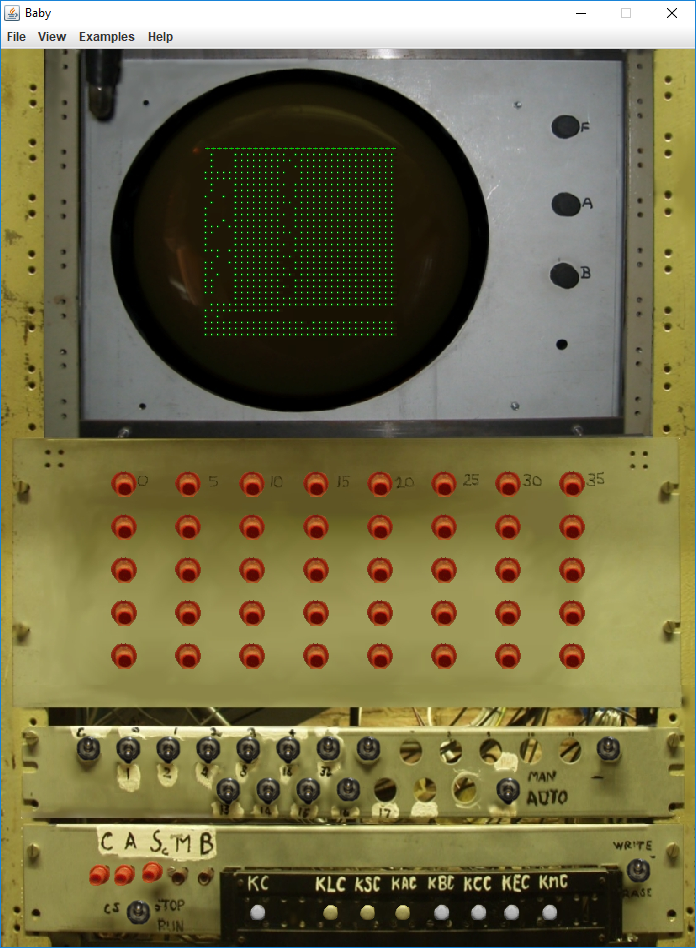
\includegraphics[width=0.5\linewidth]{images/baby-emu}
	\caption{Manchester Baby Simulator by David Sharp \citep{Baby08}. Image shows the photo-realistic interface of the emulator and its forms of input, as well as its monitor for output.}
	\label{fig:baby}
\end{figure}

The Manchester Baby was another early computer, which has its functionality described by \citet{BabyGuide08}. It was the first electronic stored program computer in the world, running its first program in 1948 before the Pilot ACE and the EDSAC. Its memory is made up of 32 store lines, each containing 32 bits. In one store line, bits 0-4 represent the operand line, i.e. the number of the line that the instruction will operate on when executed, and bits 13-15 represent the function number, which is essentially the instruction opcode.

The control of the Manchester Baby contains two values: the control instruction (CI) and the present instruction (PI). The CI contains the line number of the instruction executed previously. The PI contains the line representing the instruction currently being executed. Input can also be controlled using the switches on the front panel. Output can be displayed through the monitor above the control panel.

Regarding this emulator of the Manchester Baby, the creator chose to make it photo realistic, so it resembles the interface of the original Manchester Baby. While this is a faithful recreation, the interface feels slightly more intimidating to use than the other emulators used so far. For this reason, it would probably be better to recreate the DEUCE using a cleaner interface rather than faithfully restoring the interface as above.
The toolbar of this emulator provides control so the user can load different example programs and view the different parts of the computer, such as the store, the control, the accumulator and the disassembler. The examples tab is a useful way of loading in new programs easily so new users can quickly learn how to use the machine. It would be beneficial to replicate a feature such as this in a DEUCE emulator.

\section{Summary}
In carrying out background research, this allowed for the discovery of how the DEUCE functioned compared to modern computers and what makes for a good emulator of an early computer. Overall, the design of the DEUCE emulator for this project would be similar to the Pilot ACE emulator, as the two original computers shared much of the same design. However, all of the emulators researched require installation on a Windows PC, which limits the number of people who can access them. A better solution for a modern emulator would be to therefore make the emulator available to as many people as possible. Using this research, this also allowed for the creation of formal requirements as specified in Chapter 3.

%==================================================================================================================================
\chapter{Analysis/Requirements}
This chapter examines the process of analysing how to create the DEUCE emulator. The scope of the project is discussed, as well as the requirements gathered to create the emulator.

\section{Platform selection}
The original title assigned to this project was "Emulating Glasgow's First Computer on your Phone", but after considering several factors concerning the feasibility of creating a mobile emulator, it was agreed instead to make a web application. Firstly, it would have been extremely difficult to recreate a faithful DEUCE emulator on mobile devices given the limitations of mobile device screen sizes. For example, the DEUCE's Input Dynamisciser was a row of 32 switches, so trying to create a good interface for this on a mobile device would have been beyond the scope of this project.

Furthermore, creating this emulator as a web application is a modern solution to making the DEUCE accessible to a wide number of people. By hosting the emulator on a website, users can access it through their web browser on any device, including desktop or mobile. Therefore, the decision to change the scope of the project early on was important in order to recreate the DEUCE as faithfully as possible.

\section{Requirements Gathering}
Requirements elicitation was an important early step in the Analysis stage of the project. This helped to define what could feasibly be completed within the scope and time frame of the project. Initial general requirements were firstly created. They are as follows:
\begin{enumerate}
	\item Replicate physical features of the DEUCE, such as delay lines, card reader etc., within a modern software solution.
	\item Have a graphical user interface resembling that of the original DEUCE
	\item Allow users to interact with input switches, most likely through a pointing device.
	\item Read in programs written as "punch cards".
	\item Execute programs in the same way as the original DEUCE.
	\item Display output through representations of lights on console.
	\item Be intuitive enough for those familiar with the DEUCE to be able to operate it.	
\end{enumerate}

While these requirements sufficed as early, broad requirements, it was necessary to then refine them and categorise them into functional and non-functional requirements.

\subsection{Functional Requirements}
The functional requirements of the project define what features DEUCE emulator should have. These were categorised into Must Have, Should Have, Could Have and Want to Have requirements, using the MoSCoW method \citep{Moscow14}. They are as follows:
\\

\textbf{\textit{Must Have:}}
\begin{enumerate}
	\item A row of 32 Input Dynamiciser switches, to allow for single instruction and data input.
	\item A row of 32 Input Dynamiciser lights, to display the status of the Input Dynamiciser.
	\item A row of 32 Output Staticiser lights, to display output from instructions.
	\item A memory storage system comprised of 12 Delay Lines, 4 Temporary Stores, 3 Double Stores and 2 Quadruple Stores. These must store the following:
	\begin{enumerate}
		\item Delay Lines must store 32 32-bit words each.
		\item Temporary Stores must store 1 32-bit word each.
		\item Double Stores must store 2 32-bit words each.
		\item Quadruple Stores must store 4 32-bit words each.
	\end{enumerate}
	\item A clock to simulate delay line acoustic pulses, which are needed to access delay line memory.
	\item An instruction decoder that calculates the NIS, Source, Destination, Wait, Timing and Go values of an instruction.
	\item A single shot switch to execute a single instruction.
	\item A graphical user interface resembling that of the original DEUCE.
	\item A series of special Source and Destination addresses, as follows:
	\begin{enumerate}
		\item Source 0 - Take user input from Input Dynamiciser.
		\item Source 23 - Divide contents of TS14 by 2 and place in selected destination address.
		\item Source 24 - Multiply contents of TS14 by 2 and place in selected destination address.
		\item Source 27 - Place 1 (UNITY) in selected destination address.
		\item Source 28 - Place $ 2^{16} $ in selected destination address.
		\item Source 29 - Place $ 2^{31} $ in selected destination address.
		\item Source 30 - Place 0 (ZERO) in selected destination address.
		\item Source 31 - Place -1 in selected destination address.
		\item Destination 25 - Add the contents of the Source address to TS13 and store result in TS13.
		\item Destination 26 - Subtract the contents of the Source address from TS13 and store result in TS13.
		\item Destination 27 - Discriminate between positive and negative numbers.
		\item Destination 28 - Discriminate between zero and non-zero numbers.
		\item Destination 29 - Display output on Output Staticiser.
		
	\end{enumerate}
\end{enumerate}

\textbf{\textit{Should Have:}}
\begin{enumerate}
	\item A single shot dial to execute a given number of single shots in succession.
	\item A card reader to take external input from a pre-written DEUCE program.
	\item A card punch to write programs to external files.
	\item A Clear ID switch to clear the Input Dynamiciser lights to 0.
	\item A Clear Ops switch to clear the Output Staticiser lights to 0.
	\item A Clear Store switch to clear all data held in delay line storage.
	\item A Read and Single Read switch to read in punch cards.
	\item A Punch switch to write to output files.
	\item An Initial Input switch to read a new program.
	
\end{enumerate}

\textbf{\textit{Could Have:}}
\begin{enumerate}
	\item A user manual to instruct users on how to operate the DEUCE.
	\item A more convenient way of viewing the current memory contents of the DEUCE. While not an original feature of the DEUCE, this could help new users to view the state of their programs.
	
\end{enumerate}


\textbf{\textit{Want to have:}}
\begin{enumerate}
	\item A monitor to display output. This requirement would be extremely challenging to implement within the scope of this project and so will not be included this time.
	\item A subroutine library. The original DEUCE came with a large library of subroutines to be used by DEUCE programmers but this would be too much to implement within the time frame of the project.
\end{enumerate}
\subsection{Non-functional Requirements}
The non-functional requirements of the project describe how the emulator should work, rather than describing what the emulator will do. 
\begin{enumerate}
	\item The emulator should be easy enough to understand how to operate for those familiar with the DEUCE.
	\item It should be intuitive so that new users can learn how to operate a DEUCE.
	\item It should be designed mainly for desktop computer users but also be available on other devices such as tablets and mobile phones.
	\item It should be maintainable so that development can be continued in future.
	\item It should be able to be used as a tool to aid learning about early computers.
\end{enumerate}

\section{Summary}
This chapter gives an overview of the steps taken during the Analysis stage of the development of the project. The decision to change the project scope from being a mobile development project to a web development project was highly important, as it showed the steps taken to calculate the feasibility of the project on web compared to mobile. This stage was also key in the development process as it involved the creation of formal requirements for the project. Following these requirements would prove highly important for the rest of the project.

%==================================================================================================================================
\chapter{Design}
This chapter examines the design of the DEUCE emulator. The design of the emulator can broadly be split into two parts: the system architecture and the user interface. The design of the system architecture is concerned with the logical design of the components which make up the computer, while the user interface design examines the graphical aspect of the emulator and how to present it to users.
\section{System Architecture}
Recreating the system architecture of the DEUCE entirely within software was an important step in the design process. With much of the system architecture of the original DEUCE being physical, it was necessary to consider abstract alternatives to how the system could be imitated entirely within software. The main design concepts concerning the DEUCE emulator are detailed within this section.

\subsection{Memory Storage}
The creation of the memory storage of the DEUCE emulator, as shown in Figure \ref{fig:memory-real} presented several design questions at an early stage. Firstly, the DEUCE had two levels of main memory: delay lines and registers. Access to each of these levels was different as the delay line used clock pulses to access data, whereas for Temporary Stores, access was instant. Delay lines could also hold a vast amount of words compared to registers. Furthermore, within the registers themselves, there were varying sizes between Temporary Stores, Double Stores and Quadruple Stores. Therefore, a solution was needed to represent these different levels of memory entirely within software.

An initial design solution to this problem was to use a dictionary data structure to hold each type of storage. With keys for each type of storage, this would allow a way of accessing each level of memory entirely within software. For every key, the value pair would be an array holding the number of words each type of storage could hold. For example, keys "DL1" to "DL12" would represent the 12 Delay Lines of the DEUCE and hold an array of 32 words, while "TS13" being Temporary Store 13 could hold 1 word.

Another proposed solution to this was to simply store all levels of memory within one array of "Memory" objects. Each memory object could hold a given number of words and so could be used to represent each type of storage. The index of each type of storage would have to be tracked rather than named but given the labels of each type of storage in the architecture diagram of the original DEUCE (DL1, TS13, QS17 etc.) seen in Figure \ref{fig:arch}, it would not be difficult to do so. The number of each type of storage from the labels could be simply used as indexes within the array.

For this reason, it was decided that an array would be used over a dictionary. Ultimately, using a dictionary would overcomplicate the design of memory as software and an array would be a more efficient and effective way of keeping track of memory.
\subsection{Delay Line Architecture}
Following on from the overall design of the memory storage of the DEUCE, another large design challenge regarding the system architecture of the DEUCE emulator was the design of access to the delay lines. In early computers, delay lines provided access to data using mercury and acoustic pulses. With the data constantly flowing in the mercury tanks, it was necessary to keep track of where the data was in the delay lines using minor and major cycles. One minor cycle represented one pulse, while one major cycle represented how long it took for data to flow around an entire delay line. This is why DEUCE instructions feature Wait and Timing numbers, as these numbers calculate where in the delay lines certain data will be.

Within a web application version of the DEUCE, the design of the delay line storage of the DEUCE posed a problem. Without physical mercury delay line storage available to this emulator, a suitable substitute was needed to represent this behaviour. To emulate the behaviour of minor and major cycles of delay lines, it was decided that there should be a clock to measure minor cycles. This would be designed as a counter that would increment by 1 every minor cycle. Using this counter, it would be possible to track where data was being held in each delay line. Essentially, this counter would act like a pointer to an array. This solved the design problem of using an alternative to physical delay line storage.

\begin{figure}[t]
	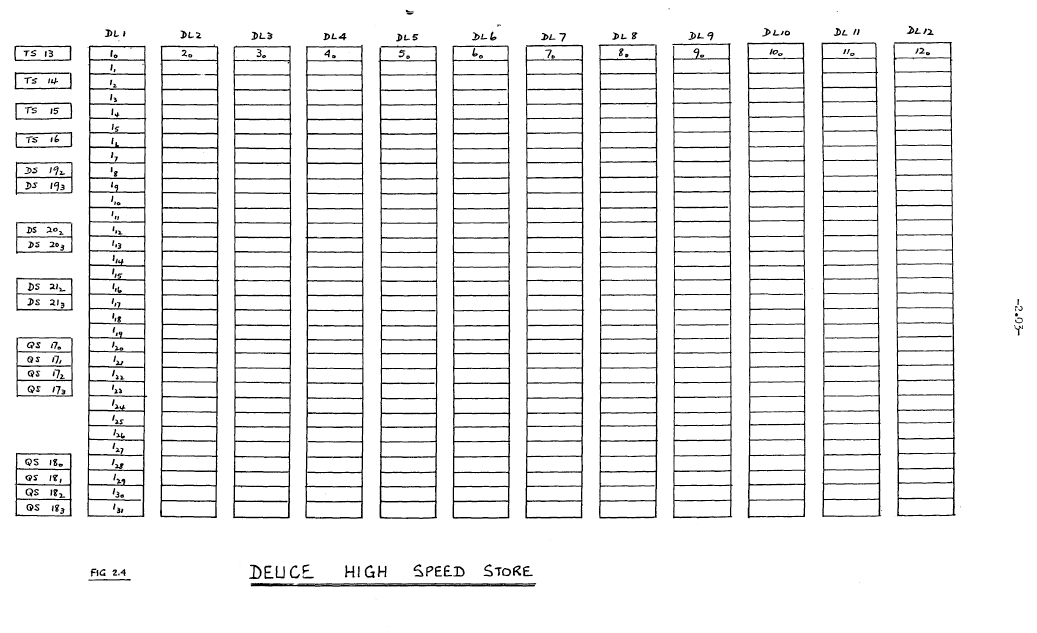
\includegraphics[width=\textwidth]{images/memory-real}
	\caption{Memory diagram of DEUCE taken from original DEUCE programming lecture notes \citep{tnmoc18}. This diagram shows the structure of memory from the original DEUCE, including the Delay Lines, Temporary Stores, Double Stores and Quadruple Stores.}
	\label{fig:memory-real}
\end{figure}

\subsection{Instruction Processing}
The design of how instructions would be processed in the DEUCE emulator was another challenging task. Each memory location in the DEUCE could hold one 32-bit word that could represent an instruction or data. As shown in Figure \ref{fig:instr-format}, a 32-bit instruction was broken down into several fields: the extra delay line bit, the NIS, the Source, the Destination, the Characteristic, the Wait, the Joe, the Timing and the Go bit. In an emulator, this would mean parsing a 32-bit number to retrieve each part of the instruction. Using these parts of the instruction, a word could be moved from one location in memory to another. The functionality of each field, as described by \citet{Vowels05}, is as follows:

\begin{figure}[h]
	\centering
	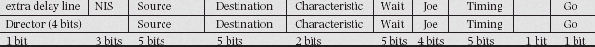
\includegraphics[width=\linewidth]{images/instr-format}
	\caption{Format of a 32-bit DEUCE instruction \citep{Vowels05}. Using each individual field, the DEUCE could be controlled to perform various actions.}
	\label{fig:instr-format}
\end{figure}

\begin{itemize}
	\item Extra delay line bit - this was set to 0 if Delay Lines 1-7 were being accessed and 1 for Delay Lines 8-12.
	\item Next Instruction Source (NIS) - this determines which delay line in memory to read the next instruction from in a program.
	\item Source - this determines the Source address of the instruction.
	\item Destination - this determines the Destination address of the instruction.
	\item Characteristic - this indicates whether or not the transfer went on for only one minor cycle.
	\item Joe - this was a spare field unused by the control unit.
	\item Wait - this delays the execution of an instruction.
	\item Timing - this indicates where in the delay line the specified instruction is to be found.
	\item Go - this is used to halt execution of a program.
\end{itemize}


\begin{figure}[h]
	\centering
	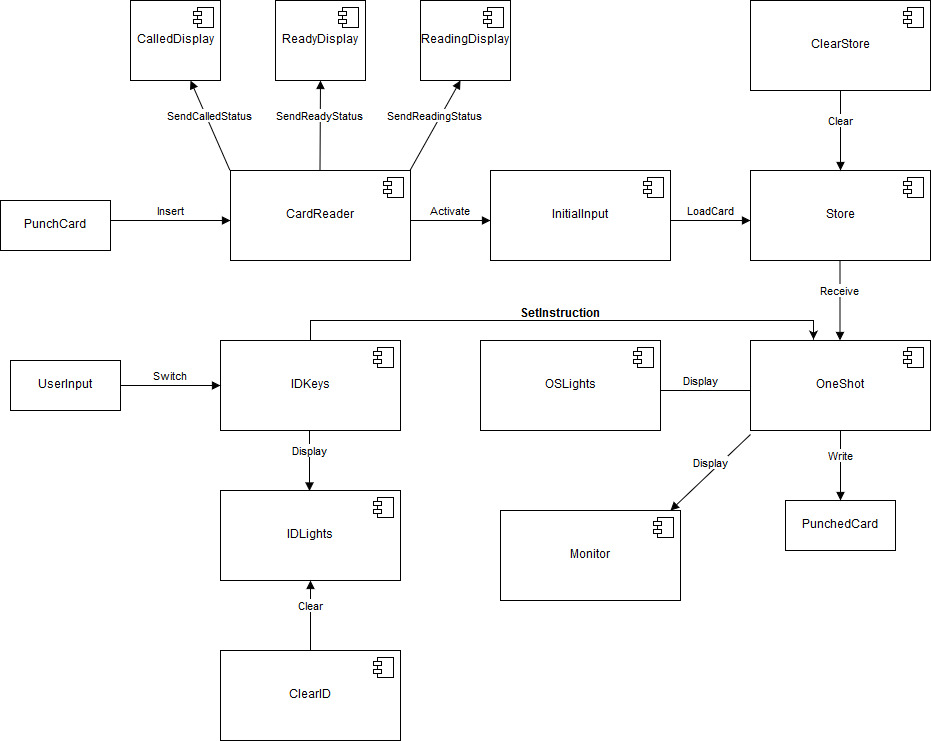
\includegraphics[width=\linewidth]{images/deuce-uml}
	\caption{Schematic diagram describing the system architecture. Input can be given via 2 sources, which is then executed via a series of single shots. On the original DEUCE, output could be given in three forms, so the project would aim to recreate this functionality.}
    \label{fig:schema}
\end{figure}
	
To help visualise the instruction processing of the emulator more clearly, a schematic diagram was created, as shown in Figure \ref{fig:schema}. This diagram was based on the description of how the DEUCE functioned in \citet{Vowels05}. The diagram shows the two forms of input a user can use to provide the emulator with data: either using a pre-written punch card, or the input switches on the console. If a punch card is entered, the card will be read in and the console will show the status of the card, either as being "Called", "Ready" or as "Being read". After the card has been read in, the Initial Input switch can be pressed to load the card into storage, so that program execution can begin. Storage can be cleared using the "clear store" switch.
	
For input via the Input Dynamiciser switches, the current state of the Input Dynamiciser will be displayed on the ID lights. These lights can be reset to 0 using the "Clear ID" switch. Each ID switch represents one bit of a 32-bit word. When the user wants to enter an instruction, they would press the "One Shot" switch to execute said instruction.
	
Regarding output, the DEUCE should display output on the Output Staticiser lights. These lights display the output of the last instruction executed as a 32-bit reverse binary word. The original DEUCE could also write output to punched cards or to the system's monitor. These features may not be implemented in this version of the DEUCE but it was important to show that these features were part of the original DEUCE architecture.

From using this diagram, the flow of program execution in the DEUCE can be seen. It identifies the key components of the DEUCE based on the functional requirements from Chapter 3.
	
\section{User Interface}
One of the key differences between the interface of the DEUCE emulator and the original DEUCE interface is the lack of hardware. Given that this project would be written entirely as software, one of they key challenges would be replicating the physical features of the DEUCE within software and representing them correctly to the user. To solve this problem, visual metaphors would need to be used to allow the user to feel as though they were using the original DEUCE.
	
The DEUCE is comprised of many switches and lights. It also features a dial to set the number of single shots to be executed in succession. While it is not possible to physically recreate these components, it is important to give the user correct feedback when operating them. To solve this challenge, it was decided that switches and lights would need to be animated properly to give the user good feedback on their actions.
	
Another large difference between a software-only DEUCE and a real DEUCE is the absence of a card reader and card punch. In the original DEUCE, a Hollerith card reader was used to read in pre-written programs and a card punch was used to physically print output on card. To replicate a card reader in a web application, a good solution would be to provide a file upload button and have users browse files to mimic inserting a program into the DEUCE. A better solution would be to use a web framework that supports "drag and drop" features, which would allow a user to "drop" a card into the card reader. 
	
For these reasons, it was necessary to select a web framework that would support these graphical needs. The selection of an appropriate web framework is later discussed in Chapter 5.

\section{Summary}
The design stage of the project was important for planning how each aspect of the project would be created. During this stage, major challenges in the design of each major component of the DEUCE were tackled, and it was decided how these challenges would be solved without reference to specific implementation. Given the complexity of the design of the original DEUCE, it was necessary to think of modern alternatives that could work within a web application. Overall, the steps taken here were very useful for the Implementation stage of the project.

%==================================================================================================================================
\chapter{Implementation}
This chapter discusses the implementation of the DEUCE emulator in terms of both front-end and back-end development. It also discusses the choice of web framework and the decisions behind this choice. 

\section{Development Tools}
Many different development tools were used to aid in the creation of the DEUCE emulator. The reasons behind choosing these tools are explained in the following sections.

\subsection{Web Framework}
The emulator was written as a web application because hosting it on the internet would allow a large number of people to access it from almost anywhere in the world. To make the emulator a suitable, modern web application, it was necessary to choose a web framework in which to create the project. Web frameworks allow for "the producibility of mature web applications with a wide range of possible features and desktop-like user interaction" \citep{kersten10}. With this in mind, three of the most popular JavaScript based web frameworks were considered to produce the DEUCE emulator: Angular \citep{angular19}, ReactJS \citep{react19} and Vue.js \citep{vue19}. JavaScript is widely used by many web applications \citep{javascript15} and would therefore be an appropriate choice of language to create this web application. Ultimately, it was decided that Angular would be chosen over the other two frameworks.

Angular is a web framework created by Google that is used for building mobile and desktop web applications \citep{angular19}. While the original version of Angular was titled AngularJS and used JavaScript, Angular in its current form uses TypeScript. However, it can still be considered JavaScript based as TypeScript shares many similarities with JavaScript and is transpiled into JavaScript when Angular applications are run in web browsers \citep{Clow18}. One of the key advantages of TypeScript over JavaScript in this project is that it is more similar to an object-oriented language such as Java than JavaScript, as it provides features such as strong typing, classes and interfaces \citep{typescript18}. An object-oriented approach, as defined by \citet{chambers14}, would be highly suitable to building this emulator as it would be a useful way to structure both the memory of the DEUCE and the graphical components for the user interface. Therefore, this gave Angular a large advantage over ReactJS and Vue.js as a choice of framework for this project.

Another advantage of Angular is that it features a large library of learning resources compared to other web frameworks. Having been built and maintained by Google, there were a vast number of tutorials and development guides compared to frameworks that are still growing, such as Vue.js \citep{vue19}. For this reason, this gave Angular another advantage as choice of web framework for this project.

\subsection{Node.js}
The Angular Command Line Interface was needed to build the emulator as an Angular application and in order for it to function properly, it was necessary to use Node.js \citep{node19}. Node is an open-source JavaScript runtime which is used as a platform for development tools and provides many reusable code modules \citep{ClowNode18}. Using the Node Package Manager \citep{npm19}, Node.js provided many useful modules for the project to be built and run.

\subsection{Version Control}
Using version control was an essential step in the implementation process, as version control "allows you to track iterative changes you make to your code" \citep{vcs16}. By using version control, it was possible for the code to be stored in a remote repository and to access a history of changes made to the code over time. For this project, GitHub \citep{github19} was used for version control. GitHub was beneficial for this project in particular because it also provided a way of hosting the project as a web application online through GitHub Pages \citep{githubpages19}. Using GitHub Pages, the project was deployed at:

 \url{https://gerardward3.github.io/level4-project/}
 
\subsection{Integrated Development Environment}
To help with writing and detecting bugs in code, an Integrated Development Environment (IDE) was necessary to use. According to \citet{ide15}, IDEs "improve developer productivity by assisting with tasks such as navigating among classes and methods, continuous compilation, code refactoring, automated testing, and integrated debugging". As this project used Angular as a framework, much of the code was written in TypeScript. For this reason, Visual Studio Code was chosen as an IDE, as "it was written by the same people who wrote TypeScript, so we know it will work well with it" \citep{visualstudio18}. It also "includes support for debugging, embedded Git control, syntax highlighting, intelligent code completion, snippets, and code refactoring" \citep{visualstudio18}. For these reasons, Visual Studio was a sensible choice as an Integrated Development Environment.

\section{Front-end development}
With the code broadly being split into "front-end" and "back-end", front-end development was started before back-end development. For the purpose of this project, "front-end" development will refer to the creation of the graphical user interface of the emulator, while "back-end" will refer to the underlying logic and behaviour of the emulator. The purpose of starting front-end development before back-end was to design a user interface that a user could load in their web browser and then make changes to each graphical component as required. 

\begin{figure}[h]
	\centering
	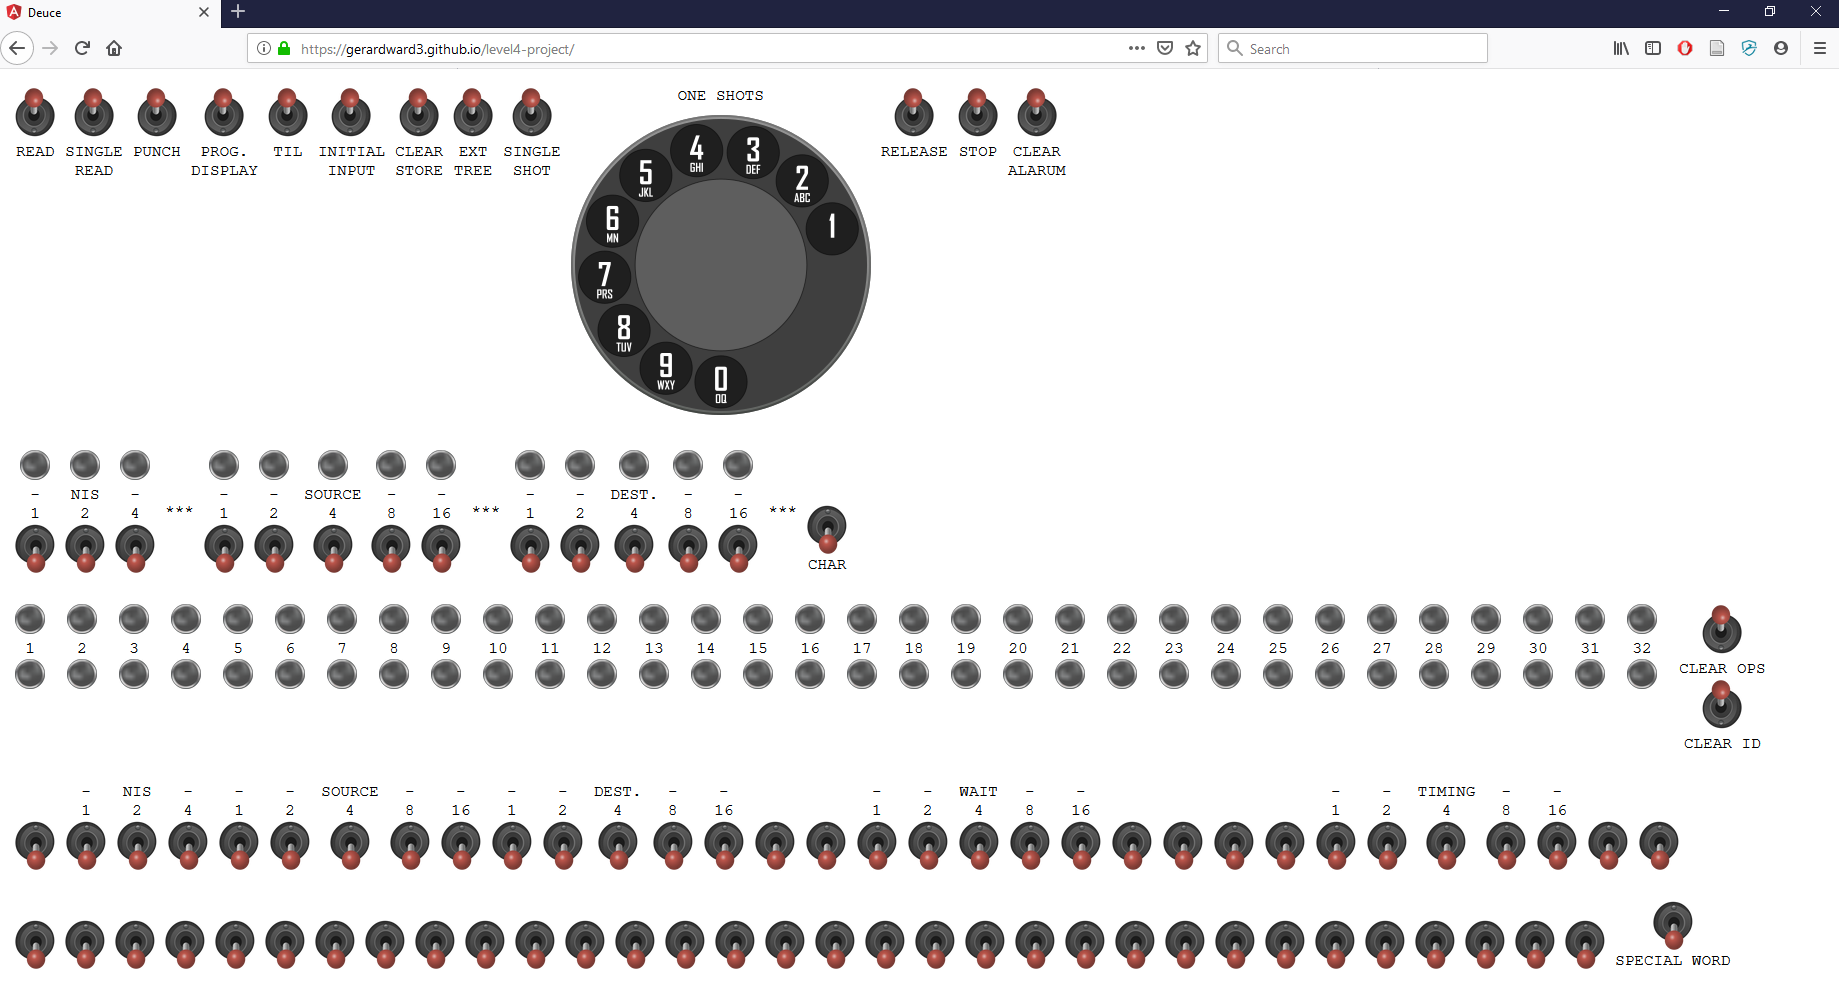
\includegraphics[width=\linewidth]{images/deuce-emu}
	\caption{Console of the DEUCE emulator loaded in a web browser. The layout of the console was based entirely on the layout of the original DEUCE console.}
	\label{fig:deuce-emu}
\end{figure}

\subsection{Graphics}
The images used in the console, as shown in Figure \ref{fig:deuce-emu} are taken from an open source library of clip art images \citep{openclipart}, under the Creative Commons Zero 1.0 Public Domain License \citep{creativecommons}. The lights and switches both have two states and show different images indicating which state they are in. This is designed to give the user feedback from their actions. The dial image is not interactive - it is there only to graphically recreate the dial on the original DEUCE panel.

\subsection{HTML and CSS}
The GUI of the emulator was written using HTML and CSS. For each type of graphical component, an Angular component was generated, providing an HTML, CSS and TypeScript file. The HTML of the overall panel features all graphical components, split up and organised using the Flexible Box Module, or Flexbox. Flexbox allows for powerful alignment controls over HTML elements using CSS. 

For each graphical component, an image path and an ID are given. The image path defines which image is to be displayed, and interacts with the TypeScript file of the component to retrieve this image. The ID is used to identify the place of the graphical component on the panel.

Switch components also feature a \texttt{click()} function in their HTML. This function listens for when a switch has been clicked and then performs an action based on the ID of the switch. For example, the when an Input Dynamiciser switch has been clicked, this is detected and in the TypeScript file for this component, its respective light is switched on.

Overall, it was important to use good HTML and CSS methods to faithfully recreate the front panel of the DEUCE. While the HTML panel of the emulator is complex due to the number of graphical components, it was important to define each of these individual graphical components with their own ID so the correct functionality could be performed. It was also important to use Flexbox to recreate the same layout as the original DEUCE.

\section{Back-end development}
The back-end development of the emulator was then carried out after a graphical user interface had been designed and deployed through Angular. This development concerned the logic of the emulator and intended to recreate the same behaviour found in the DEUCE itself.

\subsection{Memory}
\begin{figure}[h]
	\centering
	\begin{subfigure}[t]{0.45\textwidth}
		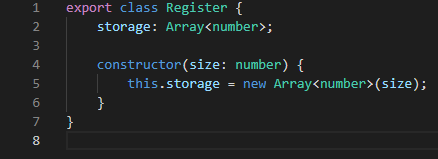
\includegraphics[width=\textwidth]{images/register-class}
		\caption{Register class from codebase. An array of numbers is created through the size parameter given in the constructor.}
		\label{fig:reg-class}
	\end{subfigure}
	\quad
	~ %add desired spacing between images, e. g. ~, \quad, \qquad, \hfill etc. 
	%(or a blank line to force the subfigure onto a new line)
	\begin{subfigure}[t]{0.45\textwidth}
		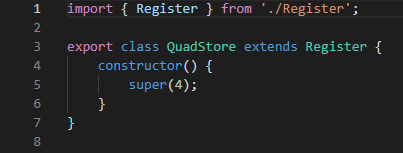
\includegraphics[width=\textwidth]{images/quad-store-class}
		\caption{QuadStore class from codebase. The QuadStore class extends the Register class to create an array of size 4. This allows it to hold 4 words, as did quad stores in the original DEUCE.}
		\label{fig:quad-class}
	\end{subfigure}
	~ %add desired spacing between images, e. g. ~, \quad, \qquad, \hfill etc. 
	%(or a blank line to force the subfigure onto a new line)    
	\caption{Excerpts from codebase of project. These show how an example of a DEUCE register is created in the emulator.}
	\label{fig:mem-classes}
\end{figure}
The memory of the DEUCE emulator was created using an object-oriented approach. Firstly, a \texttt{Register} class was created, which stores an array of TypeScript numbers of a given size in the "storage" field. Each number in this array is decimal and is then converted to a 32-bit reverse binary number when it is retrieved for use by the emulator later on. 

The \texttt{Register} class is then inherited by classes of the various levels of memory used in the DEUCE emulator: \texttt{TemporaryStore}, \texttt{DoubleStore}, \texttt{QuadStore} and \texttt{DelayLine}. Each of these classes are essentially \texttt{Register} classes with different sizes of storage. The size of the storage is determined by the value given in the super constructor of each class. For example, a \texttt{DelayLine} class gives a parameter of 32 in the super constructor while a \texttt{QuadStore} gives a size of 4 in the super constructor. This value represents the number of words each level of storage could hold in the DEUCE.

These objects then comprise a \texttt{Memory} class, which stores all levels of memory in an array and is constructed when the application is initially loaded. Index 0 of this array is set to null, as the DEUCE did not store data in memory address 0. Indexes 1 to 12 are then initialised with \texttt{DelayLine} objects, indexes 13 to 16 with \texttt{TemporaryStore} objects, indexes 17 to 18 with \texttt{QuadStore} objects and indexes 19 to 21 with \texttt{DoubleStore} objects. Using this array, the various forms of DEUCE storage can be accessed.

\subsection{Instruction Processing}
The bulk of the logic for instruction processing can be found in the \texttt{panel.component.ts} file. The \texttt{switchClicked()} function listens for when a switch is clicked on the panel of the emulator. When it detects that a switch has been clicked, it checks for the type of switch that was clicked. For example, if the switch has a corresponding light on the panel, the light which corresponds to this switch is switched on. 

Instructions given in the Input Dynamiciser are processed when it is detected that the Single Shot switch has been clicked. When this happens, the instruction is converted into a binary array of length 32 through the \texttt{readInstructionFromPanel()} function. The program then checks if it is reading in an instruction or a data value, i.e. if the previous instruction gave a Source value of 0. When it is determined that an instruction was given, the instruction is then broken down into various fields. This functionality is seen in Figure \ref{fig:process-instruction}.


\begin{figure}[h]
	\centering
	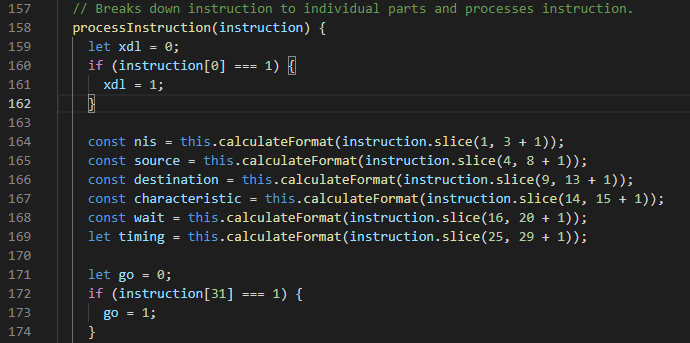
\includegraphics[width=\linewidth]{images/instruction-fields}
	\caption{Image of the processInstruction() function from emulator codebase. The fields of the instruction are calculated through the calculateFormat() function. This allows the instruction to be broken up into individual parts so the correct Extra Delay Line, NIS, Source, Destination, Characteristic, Wait, Timing and Go fields can be used to process information. The Joe field is not used as it was unused by the original control unit.}
	\label{fig:process-instruction}
\end{figure}

After being separated into individual fields, the instruction is then checked for any Source or Destination addresses that can perform special functions, such as Source 0 for a data value to be read from the Input Dynamiciser, Destination 25 for addition etc. Once these are checked, the memory transfer is performed and the Go bit is checked to discover if program execution should or should not be halted. After an instruction has been processed, the emulator then either waits on another switch to be clicked or continues with the next instruction specified through the NIS and Timing fields.

\subsection{Minor and major cycling}
While the original DEUCE used minor and major cycling to perform memory accesses to delay lines, this functionality was not captured in this emulator. The data stored in the mercury delay lines of the original DEUCE was constantly moving inside the tanks and data could be encoded through acoustic pulses in memory. To access this data, minor and major cycles were used to measure where in memory certain words were being held. An attempt at recreating this behaviour was started through the creation of a timer in TypeScript. The \texttt{dlIndex} field in \texttt{panel.component.ts} increments by 1 every half second, used to represent a minor cycle, and is then divided by 32, with its remainder being used to represent 32 minor cycles. This essentially acts as a pointer to an array and could be used in a future version of the emulator to recreate the behaviour of minor and major cycling.

\subsection{Initial Input}
While a card reader could not be implemented in this version of the emulator, a program was hard-coded into the emulator to show the functionality of how a pre-written program could be read into the DEUCE and processed. This program lights up the Output Staticiser lights from left to right from 1 to 32. The purpose of this program is to show the functionality of the NIS and Timing fields during instruction processing. Each of these fields is used to specify where in memory the next instruction is being held, so the program can continue without halting execution. The Go bit is also used to allow execution of the program to continue.

\section{Summary}
This chapter examined the technical implementation of the DEUCE emulator and the tools used to create it. Through this process, a working emulator was made and deployed. The version featured much of the functionality of the original DEUCE and its effectiveness as an emulator would go on to be evaluated, as seen in Chapter 6.

%==================================================================================================================================
\chapter{Evaluation} 
After the implementation of the project was completed, the emulator was evaluated to discover if it was a successful recreation of the DEUCE as a web application. This part of the project involved carrying out tests on various parts of the emulator to test their functionality against their corresponding parts from the original DEUCE. The emulator was also compared against the original functional and non-functional requirements defined in Chapter 2 as part of acceptance testing.

In addition, a user evaluation was carried out to gain user feedback about the emulator. The evaluation was carried out by a total of 12 participants, with half coming from a Computing Science background and half coming from a non-Computing Science background. The mix of backgrounds was chosen to evaluate if there is a difference between users who would be more likely to be proficient at using the emulator than users who would be less likely. The purpose of the overall evaluation was to determine how successful the DEUCE emulator was in being a faithful recreation of the DEUCE and to discover if it had the potential to be used as an educational tool for learning more about the DEUCE. The results of this feedback can be seen in Appendix B.

\section{Special address evaluation}
With the number of addresses used in the DEUCE for special functionality, it was important to test the special addresses implemented in the emulator to make sure they emulated the behaviour of the original. These addresses were specified in the \textit{Must Have Functional Requirements} \textbf{9.a)-m)}. The results of testing the special addresses are seen in Appendix A, with Table \ref{tab:source-instr} showing the special Source addresses and Table \ref{tab:dest-instr} showing the special Destination addresses. Every instruction that was tested successfully performed the correct function it should have, so all \textit{Must Have Functional Requirements} \textbf{9.a)-m)} were correctly implemented. These instructions also made use of an instruction decoder and single shot switch, fulfilling \textit{Must Have Functional Requirements} \textbf{6} and \textbf{7} respectively.

Several of the addresses tested only required simplistic instructions to test their functionality. Requirements \textbf{9.d)-9.h)} all followed the same program logic of placing a number in a destination address and displaying the output of the destination address. \textbf{9.m)} was evaluated in every test as it was required to display output, and functioned correctly each time. \textbf{9.a)} was also tested with a simple set of instructions, taking in input and displaying it on the Output Staticiser lights. All of these tests were straightforward and proved the functionality of their respective requirements.

Requirements \textbf{9.b)} and \textbf{9.c)} both followed the same instructions for their tests, with the only difference being the Source address in the third instruction. These tests proved that multiplication and division by two could be carried out in the emulator as it was in the original DEUCE. Similarly, requirements \textbf{9.i)} and \textbf{9.j)} followed a similar pattern, with the only difference between their test instructions being the difference in Destination addresses.

Testing requirements \textbf{9.k)} and \textbf{9.l)} proved to slightly more tricky. Discrimination in the DEUCE worked by executing one of two adjacent instructions in a delay line tank, so this was tested by firstly placing two different instructions in adjacent locations in Delay Line 3. The first instruction would display $ 2^{16} $ on the Output Staticiser, and the second would display $ 2^{31} $. The data value 1 was then sent to both Destination 27 and 28 to test \textbf{9.k)} and \textbf{9.l)} respectively. The correct output was displayed for both, proving that discrimination worked for both positive and negative numbers, and zero and non-zero numbers.

\section{Memory structure evaluation}

\begin{figure}[h!]
	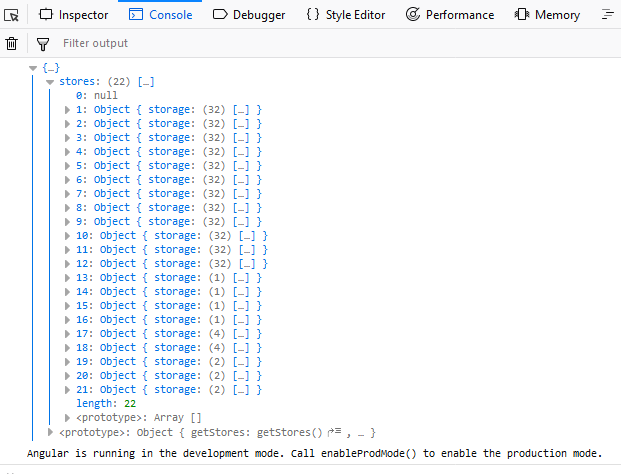
\includegraphics[width=0.9\textwidth]{images/memory-emu}
	\caption{Memory structure of DEUCE emulator shown in web browser console during development. Data structure used is an array of 22 Object arrays of varying sizes according to type of storage.}
	\label{fig:memory-emu}
\end{figure}

For data to be stored within the DEUCE emulator, the memory structure of the original DEUCE had to be replicated. In the emulator, this was successfully carried out, therefore completing \textit{Must Have Functional Requirement} \textbf{4}.

To test the memory structure of the DEUCE emulator, the Memory object created was logged to the developer console during development. This is shown in Figure \ref{fig:memory-emu}. The memory of the emulator was successfully created as an array which can hold the various levels of memory of the original DEUCE, as shown in Figure \ref{fig:memory-real}. This proves that the emulator was successful in recreating this behaviour of the DEUCE.

One part of memory that was not fully implemented was using minor and major cycling to access delay line storage. While a timer was created to measure access times, in addition to the simulation of cycling in the example program hard-coded into the emulator and executed using Initial Input, this feature was not fully integrated into the emulator. Therefore, \textit{Must Have Functional Requirement} \textbf{5} was attempted but not fully completed.


\section{User interface evaluation}

\begin{figure}[!t]
	\centering
	\begin{subfigure}[t]{0.45\textwidth}
		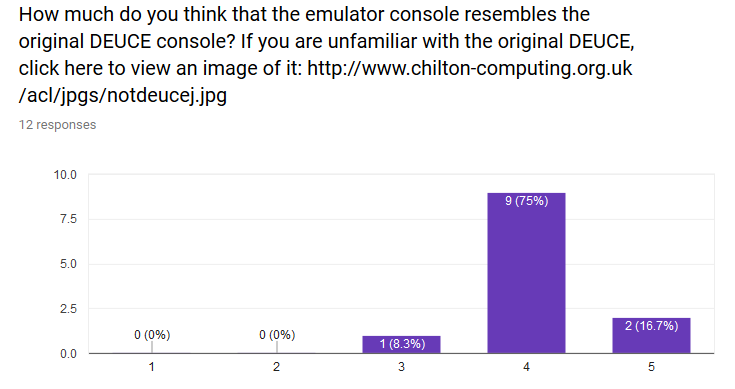
\includegraphics[width=\textwidth]{images/chart-1}
		\caption{Bar chart showing responses from User Evaluation question "How much do you think that the emulator console resembles the original DEUCE console?". The majority of respondents gave the console interface 4 out of 5 in terms of how much it resembles the original console, indicating a positive response to this question.}
		\label{fig:chart-1}
	\end{subfigure}
	~ %add desired spacing between images, e. g. ~, \quad, \qquad, \hfill etc. 
	%(or a blank line to force the subfigure onto a new line)
	\begin{subfigure}[t]{0.45\textwidth}
		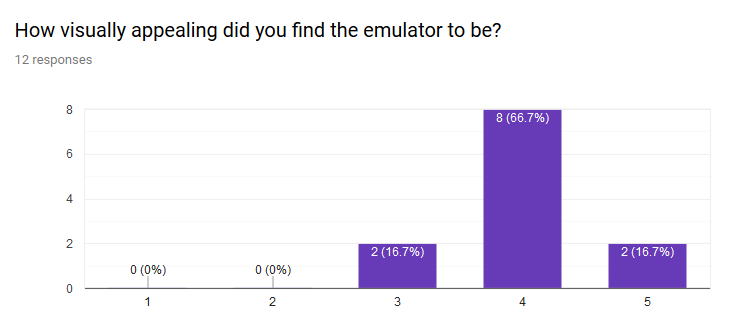
\includegraphics[width=\textwidth]{images/chart-2}
		\caption{Bar chart showing responses from User Evaluation question "How visually appealing did you find the emulator to be?" Overall, there was a positive response to this question, with the majority of respondents answering "4" on the scale from 1 to 5.}
		\label{fig:chart-2}
	\end{subfigure}
	~
	\begin{subfigure}[t]{0.45\textwidth}
		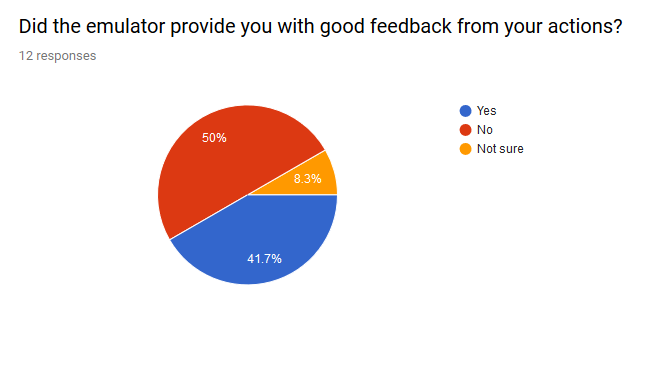
\includegraphics[width=\textwidth]{images/chart-3}
		\caption{Pie chart showing responses from User Evaluation question "Did the emulator provide you with good feedback from your actions?" Responses to this question were mixed, with 50\% of respondents answering "No" and 41.7\% of respondents answering "Yes".}
		\label{fig:chart-3}
	\end{subfigure}
	~ %add desired spacing between images, e. g. ~, \quad, \qquad, \hfill etc. 
	%(or a blank line to force the subfigure onto a new line)
	\begin{subfigure}[t]{0.45\textwidth}
		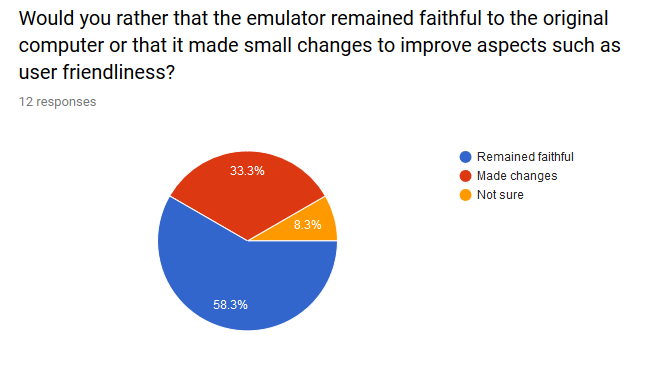
\includegraphics[width=\textwidth]{images/chart-4}
		\caption{Pie chart showing responses from User Evaluation question "Would you rather that the emulator remained faithful to the original computer or that it made small changes to improve aspects such as user friendliness?" A slight majority of 58.3\% of users said they would prefer the emulator to remain faithful over making changes.}
		\label{fig:chart-4}
	\end{subfigure}
	~ %add desired spacing between images, e. g. ~, \quad, \qquad, \hfill etc. 
	%(or a blank line to force the subfigure onto a new line)    
	\caption{Results of user evaluation from questions asked in Section 3 in survey. Questions from Section 3 were mostly concerned with questions concerning the user interface of the emulator. Overall, the emulator received positive feedback for its UI.}
	\label{fig:eval-ui}
\end{figure}

Based on both user feedback and from testing the emulator, it was concluded that the DEUCE emulator has a faithful user interface to the original DEUCE. While there was no physical DEUCE console for the emulator to be compared to, based on photos of the original DEUCE, the two console panels resemble each other. 

Many of the \textit{Should Have Functional Requirements} are present on the board but are lacking in functionality. Out of these requirements only requirements \textbf{5} and \textbf{9} were fulfilled. Given time constraints with the project, it was decided that these functions were not key to the emulator functioning at a core level, but they still should appear on the interface. Therefore, a future priority would be to implement the functionality of these graphical elements.

From the user evaluation, it is clear that users believe the user interface is faithful to the original DEUCE. In Section 3 of the user evaluation, users were asked on a scale of 1 to 5, "How much do you think that the emulator console resembles the original DEUCE console?". They were also presented with an image of the original DEUCE for comparison from \citet{chilton19}. The response, as shown in Figure \ref{fig:chart-1}, was mostly very positive, with 75\% of respondents rating the console 4 out of 5 in terms of likeness to the original console. Many users also said the console was visually appealing, with 66.7\% of respondents giving the visual appeal a 4 out of 5 rating. From this feedback, it is clear that the DEUCE emulator console was viewed as a generally faithful recreation of the DEUCE emulator and could be considered to have a good user interface.

Regarding feedback from actions when using the emulator, user responses were generally mixed, as highlighted in Figure \ref{fig:chart-3}. 50\% of respondents said they did not receive good feedback from their actions. This proved that several users found the interface to be challenging to use in terms of receiving good feedback. However, as shown in Figure \ref{fig:chart-4}, a majority of 58.3\% of users would still prefer the emulator console to remain faithful to the original console. Based on this response, this would make it difficult to alter anything in the emulator console that was not included in the original DEUCE. One respondent acknowledged that the DEUCE emulator was difficult to use because of its faithfulness to the original DEUCE, saying "The emulator seems to be true to the original computer. The system being emulated is not very user friendly and is hard to understand." (Table \ref{tab:section-3b}) This feedback conveys that the emulator was difficult to use but it was due to the difficulty of the original DEUCE console. 

\section{Usability evaluation}

\begin{figure}[!t]
	\centering
	\begin{subfigure}[t]{0.45\textwidth}
		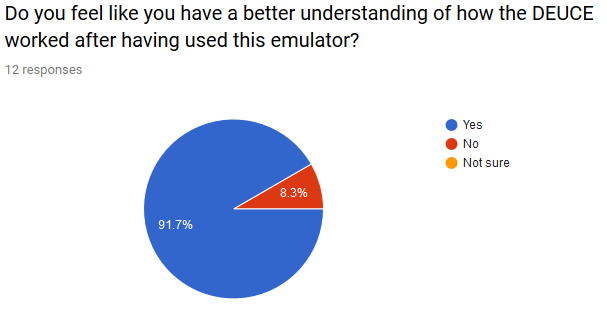
\includegraphics[width=\textwidth]{images/chart-5}
		\caption{Pie chart showing responses from User Evaluation question "Do you feel like you have a better understanding of how the DEUCE worked after having used this emulator?". Almost all users felt that they did have a better understanding after having used the emulator.}
		\label{fig:chart-5}
	\end{subfigure}
	~ %add desired spacing between images, e. g. ~, \quad, \qquad, \hfill etc. 
	%(or a blank line to force the subfigure onto a new line)
	\begin{subfigure}[t]{0.45\textwidth}
		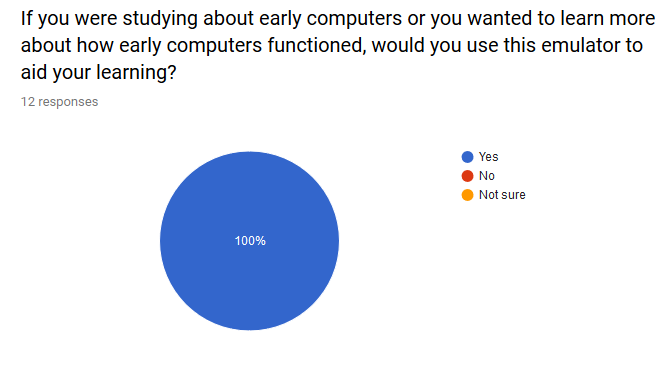
\includegraphics[width=\textwidth]{images/chart-6}
		\caption{Pie chart showing responses from User Evaluation question "If you were studying about early computers or you wanted to learn more about how early computers functioned, would you use this emulator to aid your learning?" All users said they would use the emulator as a learning aid in such a scenario.}
		\label{fig:chart-6}
	\end{subfigure}
	~
	\begin{subfigure}[t]{0.45\textwidth}
		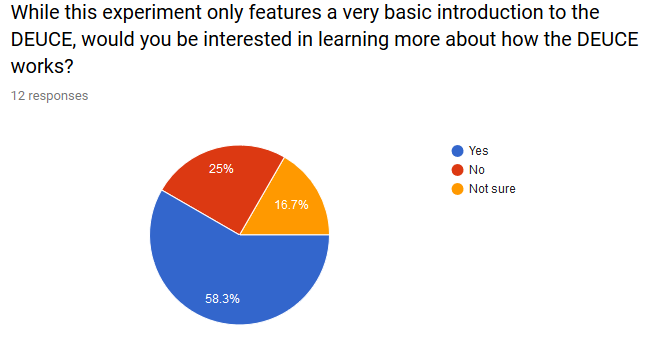
\includegraphics[width=\textwidth]{images/chart-7}
		\caption{Pie chart showing responses from User Evaluation question "While this experiment only features a very basic introduction to the DEUCE, would you be interested in learning more about how the DEUCE works?" A slight majority of users said they would be interested in learning more about it.}
		\label{fig:chart-7}
	\end{subfigure}
	~ %add desired spacing between images, e. g. ~, \quad, \qquad, \hfill etc. 
	%(or a blank line to force the subfigure onto a new line)    
	\caption{Results of user evaluation from questions asked in Section 4 of survey. Questions from Section 4 asked the user if they could see the DEUCE emulator being used as an educational tool. Overall, the vast majority of users agreed that it has the potential to be used as such a tool.}
	\label{fig:eval-usability}
\end{figure}

Another important feature of the emulator that had to be evaluated was how easy the emulator was to use and if it could be used to educate people about early computers. This was important so that new users could learn how to use the emulator but presented a problem, as the original console of the DEUCE was very complex by today's standards. 

A key inclusion that helped to make the application more usable was the creation of a user guide. While this was classified as \textit{Could Have Functional Requirement} \textbf{1}, making the user guide a lower priority requirement proved to be an error of judgement. Without the guide, users would have struggled to understand how to use the emulator, with 91.7\% of users being previously unfamiliar with the DEUCE, shown in Table \ref{tab:section-2}. This also affected \textit{Non-functional Requirements} \textbf{1} and \textbf{2}, as it is difficult to intuitively understand the DEUCE emulator without knowledge of the original DEUCE or with the help of a guide. This proved that certain requirements should have been reassessed to give them the correct priorities to aid usability.

In terms of the emulator being used as an educational tool to help teach people about early computers, many users agreed that it could be used in such a way, as shown in Figure \ref{fig:eval-usability}. 91.7\% of users felt that they had a better understanding of how the DEUCE functioned after having used the emulator. In addition, 100\% of users said they would use the emulator as a tool to aid in their learning, if they were studying about early computers. Lastly, a slight majority of 58.3\% said they would be interested in learning more about the DEUCE. This strongly indicates that the DEUCE emulator could be used as an educational tool, and so meets \textit{Non-functional Requirement} \textbf{5}. \\ \\ \\ \\ \\ \\ \\ \\


\section{Summary}
In completing the Evaluation phase of the software development process for this project, it was discovered that the DEUCE emulator could be considered a success. It meets many of its essential requirements, meeting 95\% of its \textit{Must Have Functional Requirements} and 100\% of its \textit{Non-functional Requirements}. Participants from the user evaluation also generally gave the emulator positive feedback regarding the faithfulness of the emulator to the original DEUCE and its potential as a learning tool. However, the solution was not fully completed, with only 22\% of \textit{Could Have Functional Requirements}, 50\% of \textit{Should Have Functional Requirements} and 0\% of \textit{Want to Have Functional Requirements} being met. In summary, the project successfully emulated a lot of features from the original DEUCE and could be used as a way to educate people about early computers, but more work would still be required to capture every part of the original DEUCE functionality due to its complexity.

%==================================================================================================================================
\chapter{Conclusion}    
Overall, the project of "Emulating Glasgow`s First Computer" was a success. By carrying out this project, there now exists a web-based emulator of one of the most significant early commercial computers, which allows people to use a DEUCE and learn how it functions. Unlike many other emulators of early computers, such as the ones researched in Chapter 2, this emulator was also created using a modern web framework, making it a more suitable application for today`s world than many other early computer emulators. After being evaluated by users from both Computing Science and non-Computing Science backgrounds, it was discovered that most people would use this emulator as a way of learning more about early computers. Therefore, its purpose of being used as both an educational tool and a way of preserving the legacy of the DEUCE has been achieved. 

In terms of meeting its requirements, while a lot of the key functionality of the DEUCE was recreated in the emulator, some functionality was not captured. This was mostly due to time constraints of the project and the difficulties of recreating some of the more complex aspects of the DEUCE within a modern emulator. Nonetheless, the emulator is still a faithful recreation of the original DEUCE with the functionality it currently has.

\section{Future Work}
The following sections detail what future work would be carried out on the DEUCE if there was more time and resources available.

\subsection{Minor and major cycling}
While an attempt was made at recreating the memory cycling of the DEUCE, this only resulted in a timer that would increment up to 32 every "minor cycle" then reset to 0. This timer provided the foundations for a way of providing minor and major cycling but this feature was still not properly integrated into the emulator. Consequently, finishing this feature would be one of the top priorities in a later iteration of this project.

\subsection{Additional switch and dial functionality}
Another priority regarding future work for the DEUCE emulator would be to finish implementing the functionality of the parts of the emulator console that were unable to be finished during the project. Several switches on the console, as well as the one-shot dial, have no functionality and are there purely to serve aesthetic purposes in the recreation of the DEUCE interface. Implementing these functions would allow users to use an even more faithful recreation of the original DEUCE and would be important to properly preserve the computer`s legacy.

\subsection{Additional special instructions}
Some special instructions were also not recreated in this iteration of the emulator and so, these would be logical to implement in future. For example, the instruction 7-24, which stimulates the alarum, was not featured as the emulator does not feature an alarum. Including these instructions and their corresponding features would aid in the recreation of a more faithful emulator.

\subsection{Output monitor}
The original DEUCE featured two output monitors but this was not included in this emulator. These monitors would be a very useful addition: not only would it help to recreate even more functionality of the original DEUCE, but it would implement a highly requested feature from the user evaluation. Several users asked for a better way to view the status of the program they were executing, and these monitors could be used to aid in displaying this.

\subsection{Adapting the emulator for smaller devices}
As a modern web emulator, it would be beneficial if the project could be adapted for devices with smaller screen. Currently, the DEUCE emulator is intended to be used for desktop computer use. A dilemma which arises from making the emulator responsive for mobile and tablet devices is that the original layout of the DEUCE console would inevitably be lost on smaller screens. From user evaluation, a majority of users also answered that they would rather that the emulator remained faithful to the original computer over making changes to the user interface. Therefore, it would require time to come up with a way of adapting the DEUCE for portable devices while preserving the original layout of the console.

\subsection{Further resources about the DEUCE}
The emulator is currently a single page web application which features the emulator console by itself. However, the web page could be turned into a better learning hub for the DEUCE by making additional resources available to users while they use the emulator. For example, there could be sections featuring the user guide, photos of the original DEUCE, links to other early computer emulators etc. By making these changes, this application could become one of the best sources for information about early computers publicly available on the internet. 

\section{Reflections}
From this project, I have learned a lot about several areas of Computing Science and software development. Firstly, I have gained an appreciation for how early computers functioned and how rapidly computers have developed since then. I have also learned an entirely new framework for web applications in Angular, and I could see myself using this framework again in future. Another important skill I have learned is learning how to differentiate between good and bad parts of existing similar software projects and deciding what parts to base my own project on.

While I believe the project has been a success, there are still certain things I would do differently for a project like this in future. Some of the functions missing from the emulator could have been captured had the requirements been more frequently re-assessed and if their priorities had been changed. Therefore, this reminded me of the importance of iteration in every step of the software development process. I would have also allocated myself more time for tasks in general, as too much time was taken for several steps and as a result, certain features were missing from the final product.

However, I still believe I have made a successful attempt at creating an emulator for Glasgow's first computer and I have learned much about how to develop a project of this scale individually. 


%==================================================================================================================================
%
% 
%==================================================================================================================================
%  APPENDICES  

\begin{appendices}

\chapter{Acceptance testing for special addresses}

Acceptance testing carried out for \textit{Must Have Functional Requirements} \textbf{9.a)-9.m)}. Test tables \ref{tab:source-instr} and \ref{tab:dest-instr} show what instructions were carried out for each special address in memory to test their functionality.

\begin{table}[h]
	\caption{Tests carried out against functional requirements 9.a) to 9.h). These requirements concern the special Source addresses of the DEUCE and their functionality.}
	\label{tab:source-instr}
	\begin{tabular}{|l|l|l|l|l|l|}
		\hline
		\begin{tabular}[c]{@{}l@{}}Functional \\ Requirement\end{tabular} & \begin{tabular}[c]{@{}l@{}}Address\\ and\\ function\end{tabular} & Instructions (Binary) & \begin{tabular}[c]{@{}l@{}}Instructions \\ (Source - \\ Destination)\end{tabular} & \begin{tabular}[c]{@{}l@{}}Expected \\ Output\\ (decimal)\end{tabular} & \begin{tabular}[c]{@{}l@{}}Actual \\ Output\\ (decimal)\end{tabular} \\ \hline
		9.a) & \begin{tabular}[c]{@{}l@{}}Source 0\\ - Take input \\ from Input\\ Dynamiciser\end{tabular} & \begin{tabular}[c]{@{}l@{}}00000000010110000000000000000000\\ 10100000000000000000000000000000\\ 00001011010111000000000000000000\end{tabular} & \begin{tabular}[c]{@{}l@{}}0 - 13\\ "5"\\ 13 - 29\end{tabular} & 5 & 5 \\ \hline
		9.b) & \begin{tabular}[c]{@{}l@{}}Source 23\\ - Divide\\ contents of\\ TS14 by 2\\ and place\\ in selected\\ destination\\ address.\end{tabular} & \begin{tabular}[c]{@{}l@{}}00000000001110000000000000000000\\ 00001000000000000000000000000000\\ 00001110110110000000000000000000\\ 00001011010111000000000000000000\end{tabular} & \begin{tabular}[c]{@{}l@{}}0 - 14\\ "16"\\ 23 - 13\\ 13 - 29\end{tabular} & 8 & 8 \\ \hline
		9.c) & \begin{tabular}[c]{@{}l@{}}Source 24\\ - Multiply\\ contents of\\ TS14 by 2\\ and place in\\ selected\\ destination\\ address.\end{tabular} & \begin{tabular}[c]{@{}l@{}}00000000001110000000000000000000\\ 00001000000000000000000000000000\\ 00000001110110000000000000000000\\ 00001011010111000000000000000000\end{tabular} & \begin{tabular}[c]{@{}l@{}}0 - 14\\ "16"\\ 24 - 13\\ 13 - 29\end{tabular} & 32 & 32 \\ \hline
		9.d) & \begin{tabular}[c]{@{}l@{}}Source 27\\ - Place\\ UNITY (1)\\ in selected\\ destination\\ address.\end{tabular} & \begin{tabular}[c]{@{}l@{}}00001101110110000000000000000000\\ 00001011010111000000000000000000\end{tabular} & \begin{tabular}[c]{@{}l@{}}27 - 13\\ 13 - 29\end{tabular} & 1 & 1 \\ \hline
		9.e) & \begin{tabular}[c]{@{}l@{}}Source 28\\ - Place\\ $ 2^{16} $\\ in selected\\ destination\\ address.\end{tabular} & \begin{tabular}[c]{@{}l@{}}00000011110110000000000000000000\\ 00001011010111000000000000000000\end{tabular} & \begin{tabular}[c]{@{}l@{}}28 - 13\\ 13 - 29\end{tabular} & $ 2^{16} $ & $ 2^{16} $ \\ \hline
		9.f) & \begin{tabular}[c]{@{}l@{}}Source 29\\ - Place\\ $ 2^{31} $\\ in selected\\ destination\\ address.\end{tabular} & \begin{tabular}[c]{@{}l@{}}00001011110110000000000000000000\\ 00001011010111000000000000000000\end{tabular} & \begin{tabular}[c]{@{}l@{}}29 - 13\\ 13 - 29\end{tabular} & $ 2^{31} $ & $ 2^{31} $ \\ \hline
		9.g) & \begin{tabular}[c]{@{}l@{}}Source 30\\ - Place\\ ZERO (0)\\ in selected\\ destination\\ address.\end{tabular} & \begin{tabular}[c]{@{}l@{}}00000111110110000000000000000000\\ 00001011010111000000000000000000\end{tabular} & \begin{tabular}[c]{@{}l@{}}30 - 13\\ 13 - 29\end{tabular} & 0 & 0 \\ \hline
		9.h) & \begin{tabular}[c]{@{}l@{}}Source 31\\ - Place -1\\ in selected\\ destination\\ address.\end{tabular} & \begin{tabular}[c]{@{}l@{}}00001111110110000000000000000000\\ 00001011010111000000000000000000\end{tabular} & \begin{tabular}[c]{@{}l@{}}31 - 13\\ 13 - 29\end{tabular} & -1 & -1 \\ \hline
	\end{tabular}
\end{table}

\begin{table}[h]
	\caption{Tests carried out against functional requirements 9.i) to 9.m). These requirements concern the special Destination addresses of the DEUCE and their functionality.}
	\label{tab:dest-instr}
	\begin{tabular}{|l|l|l|l|l|l|}
		\hline
		\begin{tabular}[c]{@{}l@{}}Functional \\ Requirement\end{tabular} & \begin{tabular}[c]{@{}l@{}}Address\\ and\\ function\end{tabular} & Instructions (Binary) & \begin{tabular}[c]{@{}l@{}}Instructions \\ (Source - \\ Destination)\end{tabular} & \begin{tabular}[c]{@{}l@{}}Expected \\ Output\\ (decimal)\end{tabular} & \begin{tabular}[c]{@{}l@{}}Actual \\ Output\\ (decimal)\end{tabular} \\ \hline
		9.i) & \begin{tabular}[c]{@{}l@{}}Destination 25\\ - Add the\\ contents of the\\ Source address\\ to TS13 and\\ store result in\\ TS13.\end{tabular} & \begin{tabular}[c]{@{}l@{}}00001101110110000000000000000000\\ 00001101101110000000000000000000\\ 00000111010011000000000000000000\\ 00001011010111000000000000000000\end{tabular} & \begin{tabular}[c]{@{}l@{}}27 - 13\\ 27 - 14\\ 14 - 25\\ 13 - 29\end{tabular} & 2 & 2 \\ \hline
		9.j) & \begin{tabular}[c]{@{}l@{}}Destination 26\\ - Subtract the\\ contents of the\\ Source address\\ from TS13 and\\ store result in\\ TS13.\end{tabular} & \begin{tabular}[c]{@{}l@{}}00001101110110000000000000000000\\ 00001101101110000000000000000000\\ 00000111001011000000000000000000\\ 00001011010111000000000000000000\end{tabular} & \begin{tabular}[c]{@{}l@{}}27 - 13\\ 27 - 14\\ 14 - 26\\ 13 - 29\end{tabular} & 0 & 0 \\ \hline
		9.k) & \begin{tabular}[c]{@{}l@{}}Destination 27\\ - Discriminate\\ between positive\\ and negative\\ numbers.\end{tabular} & \begin{tabular}[c]{@{}l@{}}00001101101110000000000000000000\\ 01100111011011000000000001000001\end{tabular} & \begin{tabular}[c]{@{}l@{}}27 - 14\\ 14 - 27\end{tabular} & $ 2^{16} $ & $ 2^{16} $ \\ \hline
		9.l) & \begin{tabular}[c]{@{}l@{}}Destination 28\\ - Discriminate\\ between zero\\ and non-zero\\ numbers.\end{tabular} & \begin{tabular}[c]{@{}l@{}}00001101101110000000000000000000\\ 01100111000111000000000001000001\end{tabular} & \begin{tabular}[c]{@{}l@{}}27 - 14\\ 14 - 28\end{tabular} & $ 2^{16} $ & $ 2^{16} $ \\ \hline
		9.m) & \begin{tabular}[c]{@{}l@{}}Destination 29\\ - Display output\\ on Output\\ Staticiser.\end{tabular} & \begin{tabular}[c]{@{}l@{}}00001101110110000000000000000000\\ 00001011010111000000000000000000\end{tabular} & \begin{tabular}[c]{@{}l@{}}27 - 13\\ 13 - 29\end{tabular} & 1 & 1 \\ \hline
	\end{tabular}
\end{table}
	
\chapter{Ethics checklist for user evaluation}


\begin{figure}
	\centering
	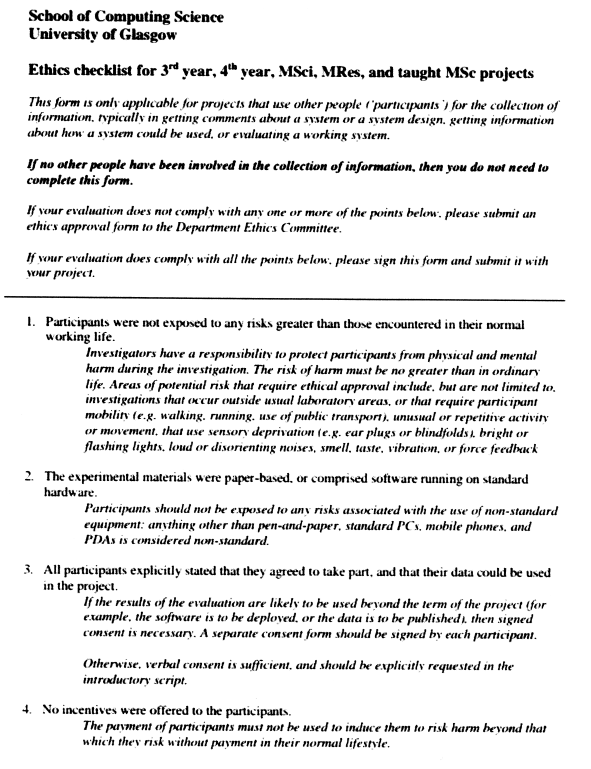
\includegraphics{images/consent-1}
	\caption{Page 1 of University of Glasgow School of Computing Science Ethics checklist.}
	\label{fig:consent-1}
\end{figure}

\begin{figure}
	\centering
	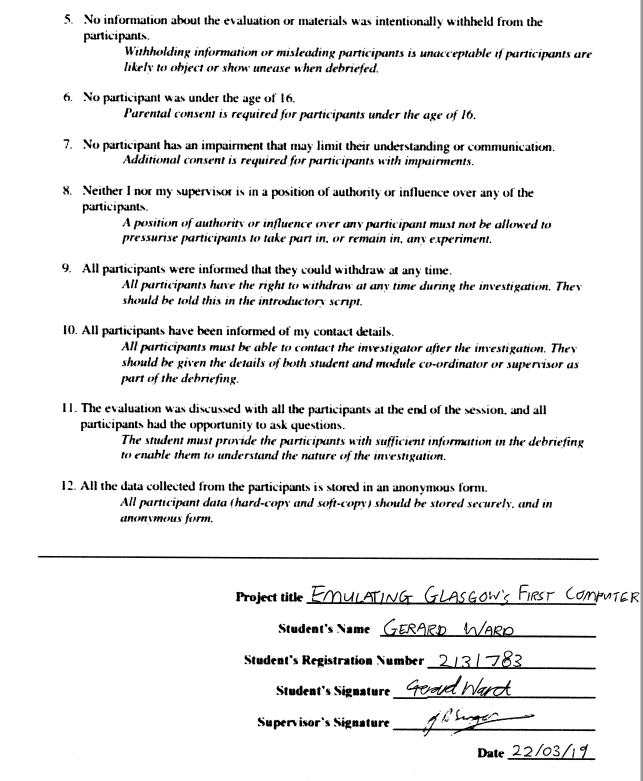
\includegraphics{images/consent-2}
	\caption{Page 2 of University of Glasgow School of Computing Science Ethics checklist.}
	\label{fig:consent-2}
\end{figure}
	
\chapter{User Evaluation}


\section{Introduction Script}
"Survey for University of Glasgow Level 4 Combined Honours Individual Project. \\
Author - Gerard Ward, 2131783, 2131783w@student.gla.ac.uk \\
Supervisor - Jeremy Singer, Jeremy.Singer@glasgow.ac.uk

Thank you for participating in this experiment. The aim of this experiment is to evaluate an emulator for the English Electric DEUCE and to discover if an emulator like this can be used as an effective tool to help people learn more about early computers. The DEUCE was one of the first commercially available electric computers in the world, and this emulator aims to replicate its behaviour as a modern web application. By gaining user feedback, the effectiveness of the emulator will be assessed.  

You will be given a link to the webpage where the emulator is hosted and a link to the user guide for the emulator. Using these, you will perform a task to execute a program on the DEUCE emulator. Afterwards, you will be asked questions about your experience using the emulator. The data you submit will be stored securely and anonymously. Using your responses, the emulator will be evaluated in terms of how well it functioned. Overall, this experiment should take around 20 minutes in total (task + survey questions).

Please remember that is it the emulator, not you, that is being evaluated. You are welcome to withdraw from this experiment at any time. If you have any questions before, during or after the experiment, please contact me at 2131783w@student.gla.ac.uk. Please answer the following questions before beginning the experiment:"

\clearpage
\section{User Evaluation - Section 1}

\begin{table}[h!]
	\caption{Table showing results for Section 1 of User Evaluation.}
	\label{tab:section-1}
	\begin{tabular}{|l|l|l|l|}
		\hline
		Timestamp & \begin{tabular}[c]{@{}l@{}}Are you \\ over the age \\ of 16? If you \\ answer No, please \\ do not continue \\ with this experiment.\end{tabular} & \begin{tabular}[c]{@{}l@{}}Do you have \\ an impairment that may \\ limit your understanding \\ or communication regarding \\ this experiment? If you \\ answer Yes, please do not \\ continue with this experiment.\end{tabular} & \begin{tabular}[c]{@{}l@{}}Do you agree to\\ take part in this \\ experiment and for \\ your data to be \\ collected anonymously \\ as part of this project? \\ If you answer No, please \\ do not continue with \\ this experiment.\end{tabular} \\ \hline
		18/03/2019 16:22:58 & Yes & No & Yes \\ \hline
		18/03/2019 20:19:00 & Yes & No & Yes \\ \hline
		19/03/2019 15:26:32 & Yes & No & Yes \\ \hline
		19/03/2019 15:30:59 & Yes & No & Yes \\ \hline
		20/03/2019 01:08:11 & Yes & No & Yes \\ \hline
		20/03/2019 14:49:38 & Yes & No & Yes \\ \hline
		21/03/2019 20:19:05 & Yes & No & Yes \\ \hline
		22/03/2019 00:18:20 & Yes & No & Yes \\ \hline
		23/03/2019 00:25:57 & Yes & No & Yes \\ \hline
		24/03/2019 14:15:39 & Yes & No & Yes \\ \hline
		24/03/2019 18:52:09 & Yes & No & Yes \\ \hline
		24/03/2019 18:58:14 & Yes & No & Yes \\ \hline
	\end{tabular}
\end{table}

\clearpage
\section{User Evaluation - Section 2}
\begin{table}[h]
	\caption{Table showing results for Section 2 of User Evaluation.}
	\label{tab:section-2}
	\begin{tabular}{|l|l|l|l|l|}
		\hline
		\begin{tabular}[c]{@{}l@{}}Have you any \\ background in \\ Computing Science \\ or Software \\ Development?\end{tabular} & \begin{tabular}[c]{@{}l@{}}If you answered \\ yes to the previous \\ question, please \\ give details below.\end{tabular} & \begin{tabular}[c]{@{}l@{}}Were you familiar \\ with the DEUCE \\ before taking \\ part in this \\ experiment?\end{tabular} & \begin{tabular}[c]{@{}l@{}}If you answered \\ yes to the \\ previous question, \\ please give \\ details below.\end{tabular} & \begin{tabular}[c]{@{}l@{}}Have you \\ used any \\ kind \\ of emulator \\ before?\end{tabular} \\ \hline
		Yes & \begin{tabular}[c]{@{}l@{}}Finishing up \\ 4th year of \\ Software Engineering\end{tabular} & Yes & \begin{tabular}[c]{@{}l@{}}Creating another\\  DEUCE emulator\end{tabular} & Yes \\ \hline
		No &  & No &  & No \\ \hline
		Yes & \begin{tabular}[c]{@{}l@{}}Studied it \\ at Advanced \\ Higher level.\end{tabular} & No &  & No \\ \hline
		No &  & No &  & Yes \\ \hline
		No &  & No &  & No \\ \hline
		Yes & \begin{tabular}[c]{@{}l@{}}4th year\\  university student\end{tabular} & No &  & Yes \\ \hline
		No &  & No &  & No \\ \hline
		Yes & \begin{tabular}[c]{@{}l@{}}Due to complete\\ 3rd Year of \\ Computing Science \\ degree at UWS \\ in 2019\end{tabular} & No &  & Yes \\ \hline
		Yes & \begin{tabular}[c]{@{}l@{}}Level 4 \\ Computing Science \\ undergraduate at \\ Glasgow.\end{tabular} & No &  & Yes \\ \hline
		Yes & Student at Glasgow & No &  & Yes \\ \hline
		No &  & No &  & No \\ \hline
		No &  & No &  & No \\ \hline
	\end{tabular}
\end{table}

\clearpage

\section{User Evaluation - Section 3a}
\begin{table}[h!]
	\caption{Table showing results for Section 3a of User Evaluation.}
	\label{tab:section-3a}
	\begin{tabular}{|l|l|l|l|}
		\hline
		\begin{tabular}[c]{@{}l@{}}Were you able \\ to successfully \\ carry out the \\ tutorial in the \\ user guide?\end{tabular} & \begin{tabular}[c]{@{}l@{}}Please give details of any parts \\ of the tutorial that you struggled \\ with.\end{tabular} & \begin{tabular}[c]{@{}l@{}}How much do you \\ think that the emulator console\\ resembles the original\\ DEUCE console? If you are \\ unfamiliar with the \\ original DEUCE, click here \\ to view an image of it: \\ http://www.chilton-computing.org.uk \\ /acl/jpgs/notdeucej.jpg\end{tabular} & \begin{tabular}[c]{@{}l@{}}How visually\\  appealing did \\ you find the\\  emulator to be?\end{tabular} \\ \hline
		Yes & \begin{tabular}[c]{@{}l@{}}I wasn't sure what I should \\ do if I had entered an instruction\\ wrong by accident so I just \\ refreshed the page and started all \\ over again\end{tabular} & 4 & 5 \\ \hline
		No & \begin{tabular}[c]{@{}l@{}}The tutorial was extremely \\ detailed and well-written. \\ However, as someone who \\ does not have a background \\ in computer science I struggled \\ comprehending when the \\ guide asked me to do \\ instructions 13 - 29 and thus \\ was unable to get the emulator \\ to work.\end{tabular} & 4 & 4 \\ \hline
		Yes &  & 4 & 4 \\ \hline
		No & The final step (6) & 5 & 3 \\ \hline
		Yes &  & 3 & 4 \\ \hline
		Yes &  & 4 & 3 \\ \hline
		Yes & \begin{tabular}[c]{@{}l@{}}I had to start the tutorial again \\ because the lights wouldn't \\ come on at  the end. \\ Worked after i tried again\\ though.\end{tabular} & 5 & 4 \\ \hline
		Yes & No issues with the tutorial itself. & 4 & 4 \\ \hline
		Yes & \begin{tabular}[c]{@{}l@{}}Understanding the \\ instruction format \\ was initially quite \\ difficult.\end{tabular} & 4 & 4 \\ \hline
		Yes &  & 4 & 4 \\ \hline
		Yes & Initial understanding & 4 & 5 \\ \hline
		Yes & \begin{tabular}[c]{@{}l@{}}Familiarising with \\ binary - after \\ understanding that \\ it went fine\end{tabular} & 4 & 4 \\ \hline
	\end{tabular}
\end{table}

\clearpage

\section{User Evaluation - Section 3b}
\begin{table}[h!]
	\caption{Table showing results for Section 3b of User Evaluation.}
	\label{tab:section-3b}
	\begin{tabular}{|l|l|l|}
		\hline
		\begin{tabular}[c]{@{}l@{}}Did the emulator \\ provide you with \\ good feedback from \\ your actions?\end{tabular} & \begin{tabular}[c]{@{}l@{}}Would you rather that\\ the emulator remained \\ faithful to the original computer \\ or that it made small changes \\ to improve aspects such \\ as user friendliness?\end{tabular} & \begin{tabular}[c]{@{}l@{}}Please give details of \\ any changes you would \\ like to see made to the \\ emulator to improve it.\end{tabular} \\ \hline
		No & Remained faithful & \begin{tabular}[c]{@{}l@{}}The right-hand panel \\ would be very useful in \\ future work as it's \\ supposed to show current \\ register values on the round\\  screens. That would be a \\ great form of feedback to \\ know whether you're switching \\ the correct switches.\end{tabular} \\ \hline
		No & Made changes & N/A \\ \hline
		Yes & Remained faithful &  \\ \hline
		No & Remained faithful &  \\ \hline
		Yes & Not sure &  \\ \hline
		Not sure & Remained faithful &  \\ \hline
		No & Made changes &  \\ \hline
		No & Made changes & \begin{tabular}[c]{@{}l@{}}The emulator seems to be true \\ to the original computer. The system \\ being emulated is not very user\\  friendly and is hard to understand. \\ Some quality of life features not \\ present in the original computer could \\ be beneficial, such as the ability\\  to flick all the switches in the \\ Input Dynamiciser off, or a \\ representation of the instructions \\ that have been previously stored.\end{tabular} \\ \hline
		No & Remained faithful & \begin{tabular}[c]{@{}l@{}}Better indication that the\\  instruction executed has\\  indeed been executed.\end{tabular} \\ \hline
		Yes & Remained faithful & \begin{tabular}[c]{@{}l@{}}It would be good if there \\ was something to tell \\ you what input you \\ had already put in.\end{tabular} \\ \hline
		Yes & Made changes & Easier way to understand output \\ \hline
		Yes & Remained faithful & \begin{tabular}[c]{@{}l@{}}None - prefer it to\\  remain as close to \\ original as possible.\end{tabular} \\ \hline
	\end{tabular}
\end{table}
\clearpage

\section{User Evaluation - Section 4}
\begin{table}[h!]
	\caption{Table showing results for Section 4 of User Evaluation.}
	\label{tab:section-4}
	\begin{tabular}{|l|l|l|l|}
		\hline
		\begin{tabular}[c]{@{}l@{}}Do you feel like \\ you have a better \\ understanding of \\ how the DEUCE \\ worked after \\ having used this \\ emulator?\end{tabular} & \begin{tabular}[c]{@{}l@{}}If you were \\ studying about \\ early computers \\ or you wanted \\ to learn more \\ about how \\ early computers \\ functioned, \\ would you use \\ this emulator to\\  aid your learning?\end{tabular} & \begin{tabular}[c]{@{}l@{}}While this experiment \\ only features a very \\ basic introduction to \\ the DEUCE, would\\  you be interested in \\ learning more about \\ how the DEUCE\\  works?\end{tabular} & \begin{tabular}[c]{@{}l@{}}Do you have any \\ \\ additional feedback\\  about the emulator?\end{tabular} \\ \hline
		Yes & Yes & Yes & \begin{tabular}[c]{@{}l@{}}I think it looks great \\ and it's a very good \\ simple introduction \\ by keeping it as simple \\ as only one instruction \\ at a time. And I like \\ that you stuck to the\\  original 32-bit instruction\\  format\end{tabular} \\ \hline
		Yes & Yes & Yes &  \\ \hline
		Yes & Yes & Yes &  \\ \hline
		Yes & Yes & Not sure &  \\ \hline
		No & Yes & Yes &  \\ \hline
		Yes & Yes & No &  \\ \hline
		Yes & Yes & No &  \\ \hline
		Yes & Yes & Yes & \begin{tabular}[c]{@{}l@{}}Even though the DEUCE \\ and by extension the \\ emulator was hard to \\ understand, through the\\  tutorial and usage of the \\ emulator I became interested\\  in the system and wanted\\  to learn more about how \\ it works, including some of \\ the other functions the system \\ is capable of beyond what was \\ explored in the user guide.\end{tabular} \\ \hline
		Yes & Yes & Yes &  \\ \hline
		Yes & Yes & Yes &  \\ \hline
		Yes & Yes & Not sure & It looks good when it lights up \\ \hline
		Yes & Yes & No & \begin{tabular}[c]{@{}l@{}}Appreciate that it has\\  remained as faithful\\  to the original as\\  possible for an \\ \\ authentic user experience.\end{tabular} \\ \hline
	\end{tabular}
\end{table}

\clearpage
\section{Debriefing Script}
"The main aim of this experiment was to evaluate an emulator for the English Electric DEUCE and to discover if an emulator like this can be used as an effective tool to help people learn more about early computers. Through this survey, I wanted to discover if users could learn how to perform very basic functions of the DEUCE using this emulator. If so, then it would be possible for this emulator to be used for more complicated functions, in order to fully replicate the behaviour of the DEUCE.

Please take a note of my email address (2131783w@student.gla.ac.uk) and the email address of my supervisor (Jeremy.Singer@glasgow.ac.uk), and please let us know if you have any further questions about the experiment. Thank you for your help."

\begin{table}[h]
	\caption{Table showing results for Section 5 of User Evaluation.}
	\label{tab:section-5}
	\begin{tabular}{|l|}
		\hline
		Do you have any comments or questions about this experiment? \\ \hline
		\\ \hline
		\\ \hline
		\\ \hline
		\\ \hline
		\\ \hline
		\\ \hline
		\\ \hline
		Impressive work, discovered a part of computing history that piqued my interest. \\ \hline
		\\ \hline
		\\ \hline
		Well thought out experiment \\ \hline
		\\ \hline
	\end{tabular}
\end{table}

\chapter{User guide}
The user guide for the DEUCE emulator is detailed in the following figures. It can also be found online at:

\url{https://drive.google.com/file/d/1Ip2_05bSA6HpiV_np4IBee1SRUu-WKop/}



\begin{figure}
	\centering
	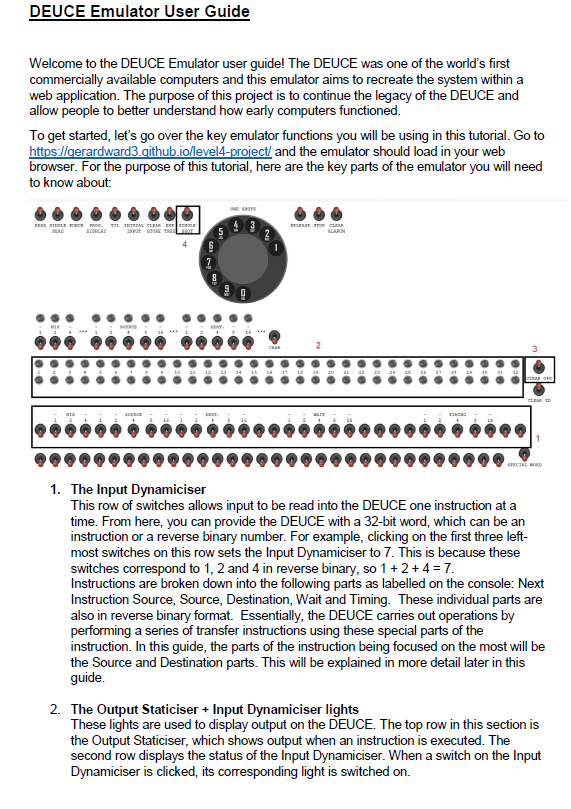
\includegraphics{images/ug-1}
	\caption{Page 1 of user guide.}
	\label{fig:pg-1}
\end{figure}

\begin{figure}
	\centering
	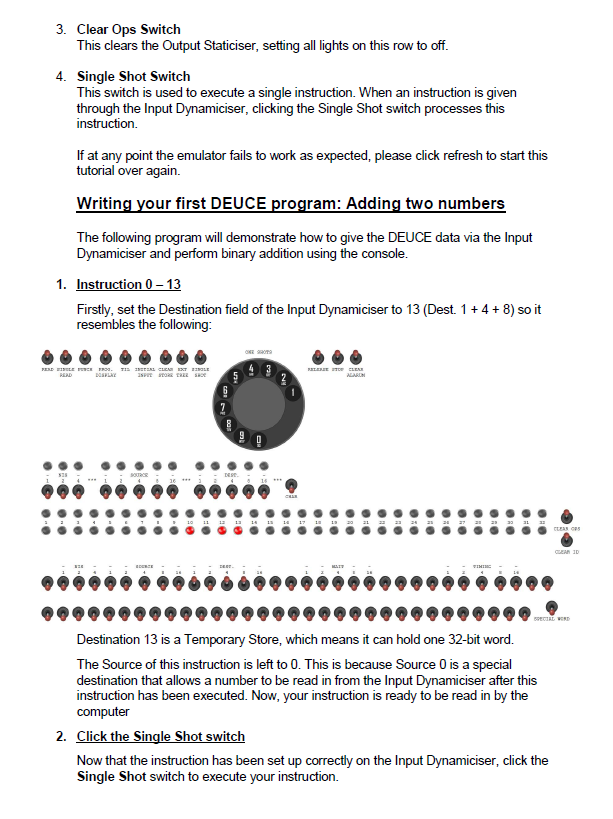
\includegraphics{images/ug-2}
	\caption{Page 2 of user guide.}
	\label{fig:pg-2}
\end{figure}

\begin{figure}
	\centering
	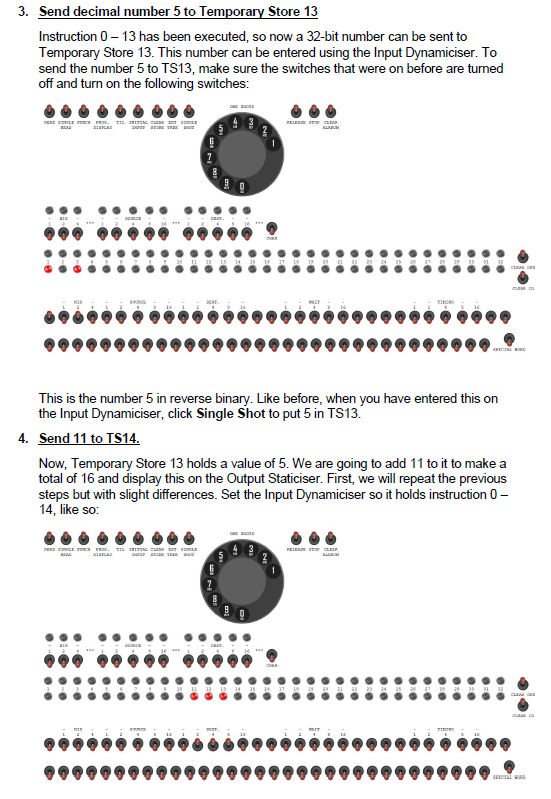
\includegraphics{images/ug-3}
	\caption{Page 3 of user guide.}
	\label{fig:pg-3}
\end{figure}

\begin{figure}
	\centering
	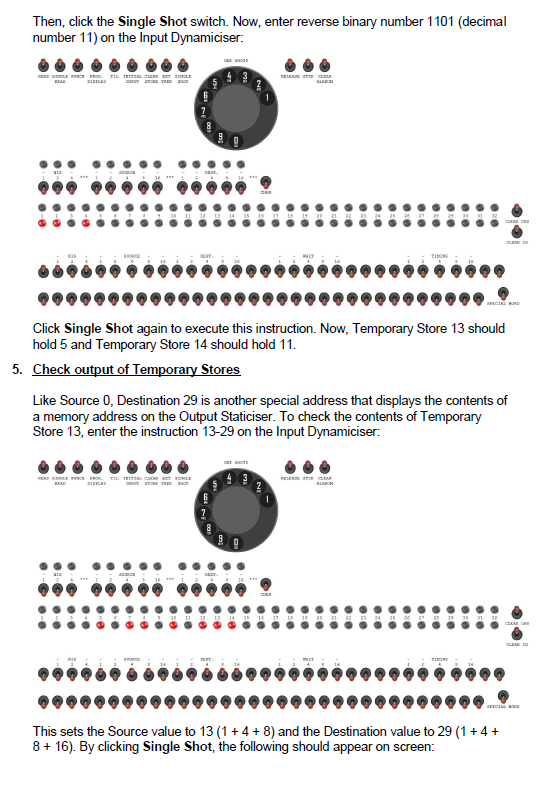
\includegraphics{images/ug-4}
	\caption{Page 4 of user guide.}
	\label{fig:pg-4}
\end{figure}

\begin{figure}
	\centering
	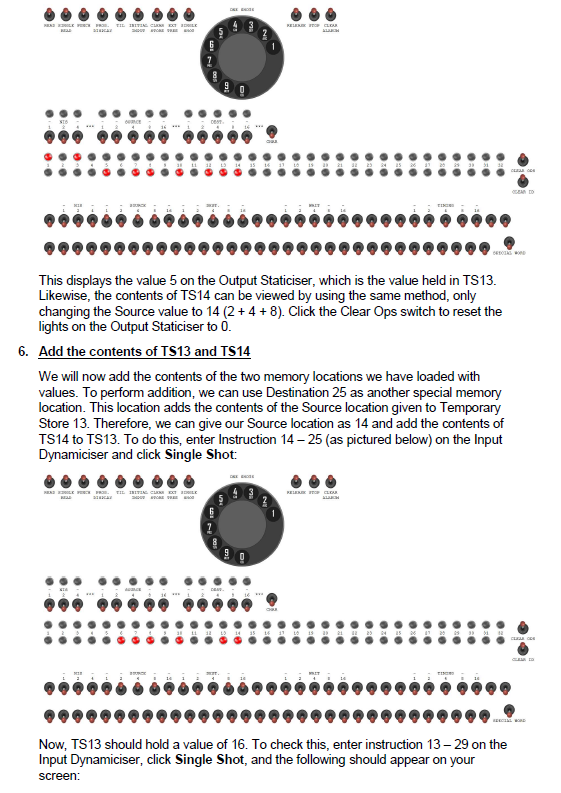
\includegraphics{images/ug-5}
	\caption{Page 5 of user guide.}
	\label{fig:pg-5}
\end{figure}

\begin{figure}
	\centering
	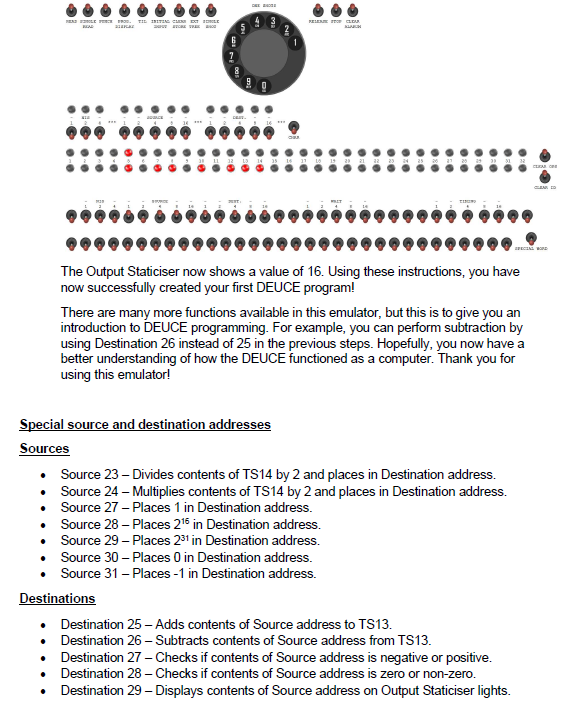
\includegraphics{images/ug-6}
	\caption{Page 6 of user guide.}
	\label{fig:pg-6}
\end{figure}

\end{appendices}

%==================================================================================================================================
%   BIBLIOGRAPHY   

% The bibliography style is abbrvnat
% The bibliography always appears last, after the appendices.

\bibliographystyle{abbrvnat}

\bibliography{l4proj}

\end{document}
